%!TEX root = P231_notes.tex

\section{Complex Analysis Review}
\lecdate{lec~12}

\subsection{Teaser: why are we doing this?}

We now switch gears to complex analysis. One of the results that I hope you'll come to appreciate in your study of physics is the rich role of complex numbers (and their generalizations) in describing nature. Our study of complex analysis will focus on motivating the residue theorem to calculate integrals in complex space. This, in turn, is useful when we represent functions in \emph{momentum space} by Fourier transforming. For example, a Green's function $G(x,x')$ can be written with respect to the Fourier momentum variable $k$ by
\begin{align}
	G(x,x') &= \int \dbar k \, e^{-ikx} \tilde G(k,x') \ ,
	\label{eq:complex:intro:G:fourier}
\end{align}
where I've used a convenient notation where $\dbar = d/2\pi$. This, in turn is useful because our defining relation for the Green's function is \eqref{eq:Greens:func:as:inverse}:
\begin{align}
	\mathcal O_xG(x,x') &= \delta(x-x') \ ,
\end{align}
which we may then write (Fourier transforming both sides) as
\begin{align}
	\mathcal O_x \int \dbar k \, e^{-ikx} \tilde G(k,x') 
	=
	\int \dbar k \, e^{-ikx} e^{ikx'} \ .
	\label{eq:complex:intro:defining:G:}
\end{align}
On the right-hand side we've written the $\delta(x-x')$ in its Fourier representation. We have assumed that $\mathcal O_x$ is a polynomial in derivatives with respect to $x$:
\begin{align}
	\mathcal O_x = \sum_{n=0}^{\infty}
	p_n(x) \left(\frac{d}{dx}\right)^n
	\equiv P\left(x,\frac{d}{dx}\right) \ .
	\label{eq:complex:intro:defining:Ox}
\end{align}
What's powerful about this is that that when we apply a differential operator in $x$ onto the Fourier representation of a function, say \eqref{eq:complex:intro:G:fourier}, then the derivatives only `see' the exponential factor $e^{-ikx}$. This means that derivatives are particularly easy:
\begin{align}
	\left(\frac{d}{dx}\right)^n e^{-ikx} &= (-ik)^n \ .
\end{align}
This means that we may write the differential operator $\mathcal O_x$ in \eqref{eq:complex:intro:defining:Ox} when it acts on the Fourier representation as
\begin{align}
	\mathcal O_x = \sum_{n=0}^{\infty}
	p_n(x) \left(-ik\right)^n
	\equiv P\left(x,-ik\right)  \ ,
\end{align}
so that the defining relation for $G$,
\eqref{eq:complex:intro:defining:G:}, may in turn be simplified:
\begin{align}
	\int \dbar k \, e^{-ikx} P(x, -ik) \tilde G(k,x') &= \int \dbar k \, e^{-ik(x-x')} \ ,
\end{align}
which suggests a simple expression for the Fourier coefficients:
\begin{align}
	\tilde G(k,x') &= e^{ikx'} \left[P(x,-ik)\right]^{-1} \ ,
	\label{eq:Greens:function:Fourier:transform:heuristic}
\end{align}
where one may find $G(x,x')$ from simply taking the inverse Fourier transform. There will turn out to be a few neat features of this approach, but before getting there, let's start from the very beginning.

\lecdate{lec~13} % or Lec 11 of 2017

\subsection{Complex Numbers}

A complex number $z$ may be decomposed into real and imaginary parts
\begin{align}
	z = x + i y \ ,
\end{align}
where $x$ and $y$ are both real numbers. We may also define the complex conjugate as
\begin{align}
	\bar z = z^* = x - i y \ .
\end{align}
One may also write these variables in a polar notation,
\begin{align}
	z &= re^{i\theta}
	&
	\bar z &= re^{-i\theta} \ ,
\end{align}
where $r \in [0,\infty]$ and $\theta \in [0, 2\pi]$:
\begin{center}
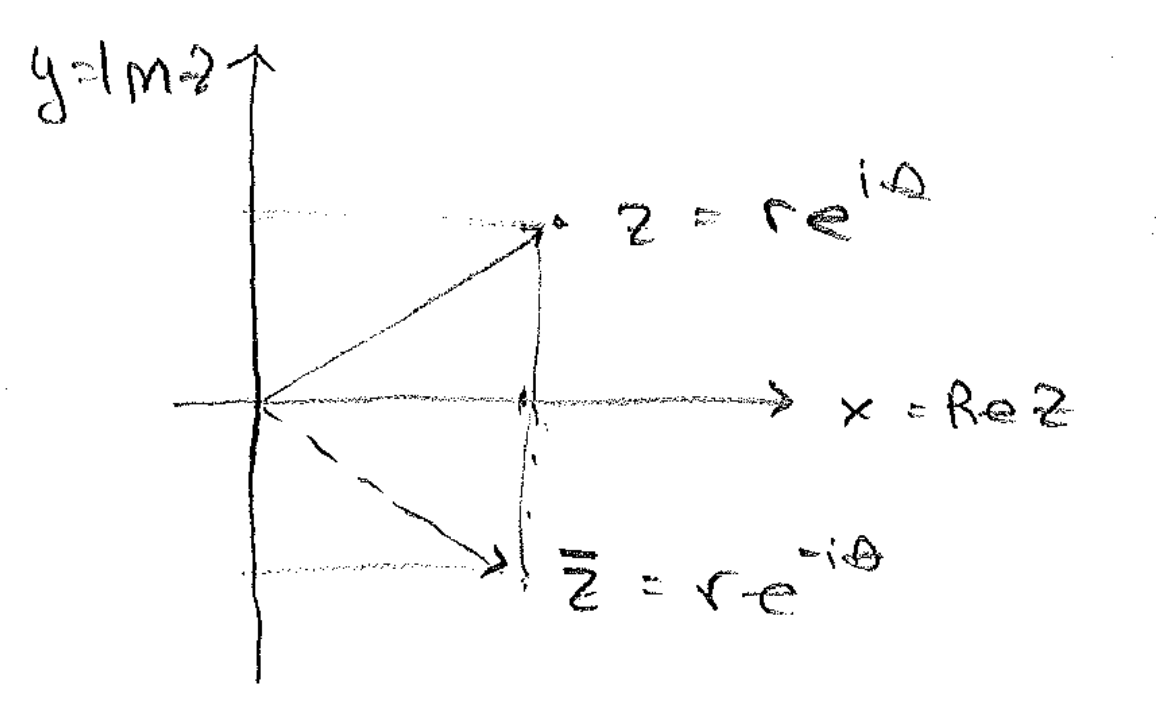
\includegraphics[width=.5\textwidth]{lec13_complexvar}
\end{center}
Complex numbers live in the space of complex numbers $\mathbbm{C}$, a \emph{two-dimensional} real space with coordinates $(x,y)$ in $\mathbbm{R}^2$ augmented by an additional rule for multiplication (take two complex numbers and return a complex number) that is called the \emph{complex structure}. This is basically the definition $i^2 = -1$, though one may generalize to higher complex dimensions. 


\subsection{Complex functions}

Complex functions take complex numbers and return complex numbers. Inspired by the two-dimensional-ness of $\mathbbm{C}$, let us write a complex function as $f(z)=f(x,y)$ where $z = x+i y$. Because $f(x,y)$ is, itself, a complex number for a given $z=x+i y$, we can decompose $f$ into two real-valued functions
\begin{align}
	f(z) = f(x,y) &= u(x,y) + i v(x,y) \ .
\end{align}
This is clearly a map from $\mathbbm{C} \to \mathbbm{C}$ and so we can simply ``do multivariable calculus'' on this space. 

If we forget the complex structure, then this \emph{seems} to simply be the calculus of maps between $\mathbbm{R}^2 \to \mathbbm{R}^2$ where
\begin{align}
	f(x,y) &= u(x,y) \hat{\vec{x}} + v(x,y)\hat{\vec{y}} \ .
\end{align}
In that case, we need to collect the partial derivatives. We know that we can write the variation of $f$ as
\begin{align}
\delta f(x,y) &= \delta u(x,y) \hat{\vec{x}} + \delta v(x,y)\hat{\vec{y}} 
=
\left(
	\frac{\partial u}{\partial x}\delta x +
	\frac{\partial u}{\partial y}\delta y
\right)\hat{\vec{x}}+
\left(
	\frac{\partial v}{\partial x}\delta x +
	\frac{\partial v}{\partial y}\delta y
\right)\hat{\vec{y}} \ .
\end{align}
Remembering our complex structure, we can write this succinctly as
\begin{align}
	\delta f &= 
	\frac{\partial f}{\partial z}\delta z +
	\frac{\partial f}{\partial \bar z}\delta \bar z \ ,
	\label{eq:complex:2D:deviation}
\end{align}
where we're using
\begin{align}
	\frac{\partial}{\partial z} &= 
	\frac{1}{2}
	\left(
	\frac{\partial}{\partial x}
	+
	\frac{\partial}{\partial (iy)}
	\right)
	&
	\frac{\partial}{\partial \bar z} &= 
	\frac{1}{2}
	\left(
	\frac{\partial}{\partial x}
	+
	\frac{\partial}{\partial (-iy)}
	\right) 
	\\
	&=
	\frac{1}{2}
	\left(
	\frac{\partial}{\partial x}
	-i
	\frac{\partial}{\partial y}
	\right)
	&
	\frac{\partial}{\partial \bar z} &= 
	\frac{1}{2}
	\left(
	\frac{\partial}{\partial x}
	+i
	\frac{\partial}{\partial y}
	\right) 
	\ .
	\label{eq:ddz:ddzst}
\end{align}
The fact that partial derivatives combine like this may be familiar\footnote{This comes from the underlying mathematical structure. The partial derivatives are basis vectors for the \emph{tangent space} at some point $(x,y)$. These partial derivatives ask: how much does the function I'm acting on change if I move by one unit in this direction?}. 

So far we have emphasized that $f(x,y)$ behaves like a function in two real dimensions. Critically, in some ways we want to think about functions $f(z)$ that are functions of `one' [complex] dimension rather than two real dimensions. In two real dimensions, calculus came with a notion of directional derivative. When we wanted the rate of change for a function, we had to ask \emph{in what direction} are we checking the rate of change. At a given function may change by a positive amount in the $x$-direction, but a negative amount in the $y$-direction, for example. This is in contrast to one-dimensional calculus where each point had an unambiguous derivative that represented how much the function changed in the positive $x$ direction with respect to a point $x_0$:
\begin{align}
	\delta f(x) = \frac{d f(x_0)}{d x} (x-x_0) + \cdots \ .
\end{align}
This is in contrast to the change in a general complex function \eqref{eq:complex:2D:deviation}. In fact, if we explicitly wrote some expansion with respect to a point $z_0$, it looks a little funny:
\begin{align}
	\delta f(z) &= 
	\frac{\partial f}{\partial z}(z-z_0) +
	\frac{\partial f}{\partial \bar z}(\bar z-\bar z_0) + \cdots \ .
\end{align}
What is going on here? Why should $f(z)$ be a function of one complex variable $z$ but the expansion seems to depend not only on $(z-z_0)$ but also $(z-z_0)^*$?

\subsection{Analytic complex functions are nice}

This leads us to a definition of ``nice'' complex functions. The following terms are all more-or-less equivalent for this sense of nice-ness: \textbf{[complex] differentiable}, \textbf{analytic}, \textbf{holomorphic}, \textbf{regular}. This is simply the restriction that the $\partial f/\partial \bar z$ term should vanish so that the variation $f(z)$ only depends on $\delta z$ and not $\delta\bar z$. In other words, an analytic function admits usual single-dimensional definition of the derivative,
\begin{align}
	\frac{df(z_0)}{dz} &= \lim_{z\to z_0} \frac{f(z)-f(z_0)}{z-z_0} \ .
	\label{eq:df:dz:analytic:def}
\end{align}
The key aspect of this is that there is only \emph{one} value of $df/dz$ at $z_0$ no matter how you approach $z_0$. In other words, it doesn't matter if $\delta z = z-z_0$ is coming from the positive/negative real/imaginary direction. The value of $df/dz$ is the same. 

For most of these lectures we will use the term \textbf{analytic} to refer this property. Let us see what happens when we impose $df/d\bar{z} = 0$ onto the component functions $u(x,y)$ and $v(x,y)$:
\begin{align}
	\frac{1}{2}\left(\frac{\partial}{\partial x} + i \frac{\partial}{\partial y}\right)
	\left[u(x,y)+iv(v,y)\right]
	&= 
	\frac{1}{2}
	\left( \frac{\partial u}{\partial x} - \frac{\partial v}{\partial y} \right)
	+
	\frac{i}{2}
	\left( \frac{\partial u}{\partial y} + \frac{\partial v}{\partial x} \right)
	= 0 \ .
\end{align}
This implies the \textbf{Cauchy--Riemann equations}, which are equivalent to the function $f$ being analytic:
\begin{align}
	\frac{\partial u}{\partial x} & = +\frac{\partial v}{\partial y}
	&
	\frac{\partial u}{\partial y} & = -\frac{\partial v}{\partial x} \ .
\end{align}

Thus far we've talked about functions being analytic or not. It turns out that analytic functions are \emph{so} nice that there really aren't that many physically relevant functions that are analytic \emph{everywhere}\footnote{The analog here is people who are nice. Most people are nice most of the time. But very few people are nice \emph{all} of the time. I suspect Fred Rogers may be one of the few who could plausibly be \sout{analytic} \emph{nice} everywhere.}. Instead, we will often talk about functions that are analytic in most places but are not analytic (differentiable) in other places. Indeed, the \emph{non}-analyticity of Green's functions is a key result in this class.

\subsection{Analyticity is Differentiability}

We have motivated the Cauchy--Riemann equations from the notion of being independent of $z^*$. This is a useful crutch and fits our theme of motivating rather than rigorously proving results. Let us be clear, however, that the underlying definition of analyticity is that:
\begin{quote}
a function that is analytic at a point $z_0$ is differentiable at $z_0$.
\end{quote}
A function is differentiable at a point $z_0$ if its derivative, \eqref{eq:df:dz:analytic:def}, has a well-defined \emph{finite} value. A function that is itself infinite at a point cannot have a well-defined limit \eqref{eq:df:dz:analytic:def}, and thus are \emph{not} analytic at that point.
We distinguish this from $df/dz^*=0$ because of the importance of \emph{singular} functions in physics. 
\begin{example}
The following function is non-analytic at $z=2i$ and $z=1$:
\begin{align}
	f(z) = \frac{3z}{(z-2i)(z-1)} \ .
\end{align}
It may seem like $df/dz^* = 0$ at these points because $f(z)$ is independent of $z^*$. However, one cannot say that $df/dz^*=0$ because the limit definition analogous to \eqref{eq:df:dz:analytic:def} is not defined. 
\end{example}
\begin{exercise}
The notion of `independent of $z^*$' sometimes causes more confusion than its worth. After all, $z$ and $z^*$ are clearly \emph{not} independent variables. Given $z$, you know exactly what $z^*$ is. The notion in which we \emph{pretend} that $z$ and $z^*$ are independent is that
\begin{align}
	\frac{\partial z}{\partial z^*} = 
	\frac{\partial z^*}{\partial z} = 0 \ ,
\end{align}
which we understand to come from an interpretation of $\mathbbm C \sim \mathbbm R^2$. Use \eqref{eq:ddz:ddzst} to prove the above partial derivative relations.
\end{exercise}



\subsection{A geometric point of view (optional)}
\label{sec:analytic:geometric}

For culture, let us comment on a geometric perspective of analyticity/complex-differentiability. The differential of a function, $df$, is a \textbf{differential one-form}. If you recall some of our nomenclature for dual vectors, a one-form is a kind of `row vector': it is a linear function that takes in a vector and spits out a number. If $df$ is such a dual vector, what is the vector space upon which it acts?

Let's specifically consider the differential of $f$ at a specific point $z_0$ in the complex plane: $df(z_0)$. This is not a number. In order to get a number from this, you have to feed it a vector: I claim this vector is an element of the tangent plane\footnote{The tangent plane is exactly what it sounds like: if you have a curved surface like a globe, the tangent plane at $z_0$ and glued a rigid piece of cardboard to one point, $z_0$. Now imagine that the piece of paper has graph paper on it.} of the complex plane at $z_0$: $T_{z_0}\mathbbm{C}$. We can sketch this if you allow me to artificially `curve' the complex plane to help make it easy to distinguish:
\begin{center}
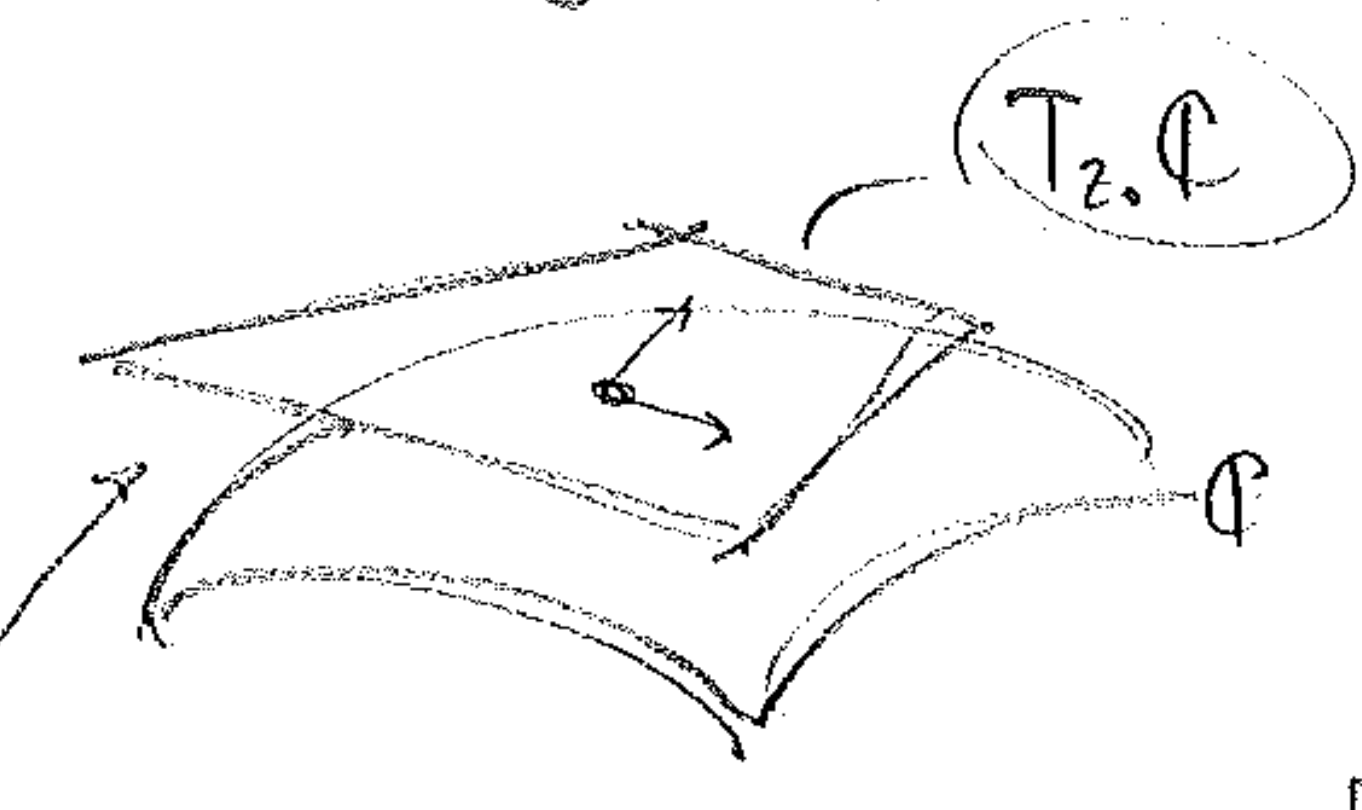
\includegraphics[width=.5\textwidth]{figures/lec13_mani.png}
\end{center}
Using the jargon of differential geometry, we call the complex plane the \emph{base manifold}. The set of all tangent spaces is called a \emph{tangent bundle}\footnote{More general types of vector spaces can be attached to each point of the base manifold. These are called fiber bundles. They are the underlying mathematical structure of mechanics and reflect why Hamilton's equations are so damn special. They are also the mathematical structure that defines gauge theories and so address the question ``what is a force?''}. Each tangent space is a vector space `attached' to a single point of the base space. 

The object $df(z_0)$ is a dual vector on the vector space\footnote{The standard notation is to write a dual vector of a space $V$ as a vector in the dual space $V^*$, so one could write $df(z_0) \in T^*_{z_0}(\mathbbm{C})$.} $T_{z_0}(\mathbbm{C})$.  The vectors of this space are `velocities' of trajectories that pass through $z_0$. For now let's think of them as quantities
\begin{align}
	\vec v = \Delta x + i \Delta y \ .
\end{align}
\begin{center}
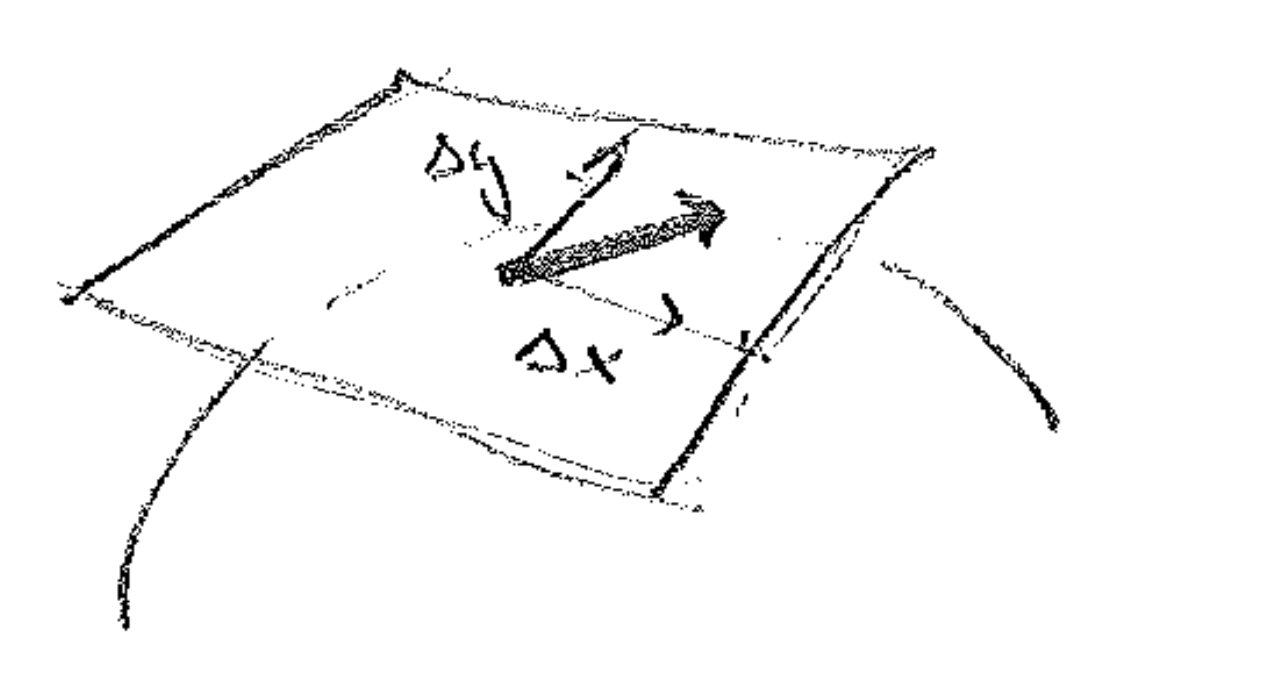
\includegraphics[width=.5\textwidth]{figures/lec13_tanvec.png}
\end{center}
Then we may write the linear action of $df(z_0)$ on $\vec v \in T_{z_0}(\mathbbm{C})$ as
\begin{align}
	df(z_0)\left[\vec{v}\right] &=
	f'(z_0)\Delta x + f'(z_0)i\Delta y \ ,
	\label{eq:diff:geo:CR:1}
\end{align}
where we assume that $f$ is analytic so that $f'(z_0)$ is unambiguously defined (independent of the direction of $\delta z$) as in \eqref{eq:df:dz:analytic:def}. 

However, if we think about this complex space as a two-dimensional real space, the following is also true:
\begin{align}
	df(z_0)\left[\vec{v}\right] &=
	\left.\frac{\partial f}{\partial x}\right|_{z_0} \Delta x
	+
	\left.\frac{\partial f}{\partial y}\right|_{z_0} \Delta y
	\label{eq:diff:geo:CR:2}
\end{align}
Comparing \eqref{eq:diff:geo:CR:1} and \eqref{eq:diff:geo:CR:1} gives 
\begin{align}
	\frac{\partial f}{\partial x} = f'(z_0) = - i\frac{\partial f}{\partial y} \ .
\end{align}
Recalling that $f= u+iv$ then gives
\begin{align}
	\frac{\partial u}{\partial x}
	+ i
	\frac{\partial v}{\partial x}
	=
	-i
	\frac{\partial u}{\partial y}
	+
	\frac{\partial v}{\partial y} \ .
\end{align}
Setting the real and imaginary parts equal to one another give, as expected, the Cauchy--Riemann equations. 

\subsection{Analytic and harmonic}

One more comment is in order. If a function $f(z) = u(x,y)+ i v(x,y)$ is analytic, then its real and imaginary parts are independently 2D harmonic with respect to $\mathbbm{R}^2$:
\begin{align}
	\partial_x^2 u(x,y) + \partial_y^2 u(x,y) &= 0
	&
	\partial_x^2 v(x,y) + \partial_y^2 v(x,y) &= 0 \ .
\end{align}
Harmonic functions show up all over the place---though admittedly you probably care mostly about three-dimensional harmonic functions. The above realization may be helpful, however, for 3D systems for which the third dimension is trivial. For example, you may want to consider fluid flow across an airplane wing. One can take the limit where the wing is infinitely long so that the fluid dynamics reduces to the two-dimensional motion around a cross section of the wing. Alternatively, maybe you care about an electrostatic system which are similarly `effectively' 2D. In this case you can `promote' your real harmonic variable (a fluid dynamics potential or electrostatic potential) to an analytic function and then bear the full power of complex analysis to attack the problem. One of the most fascinating---if outdated---methods is called \textbf{conformal mapping} by which one can solve for a harmonic function with weird boundary conditions by mapping to much simpler boundary conditions. This topic is beautiful and gives a first, intuitive example of \emph{conformal transformations} which are a pillar of theoretical physics (in any discipline). The technique is how engineers in the pre-personal computer era designed airplane wings. For experimentalists, it is pretty neat that \acro{UCR}'s own Nathan Gabor has created an analogous micromagnetic `solver' of this very same problem\footnote{\url{https://arxiv.org/abs/2002.07902}}.

\subsection{Complex functions as maps}

A complex function $f(z)$ takes in a complex number and returns a complex number. These are maps of the complex plane to itself. It is useful to build an intuition for this rather trivial-sounding statement: complex functions `deform' the complex plane. 

\begin{example}
Consider the function that multiplies a complex number by a constant phase,
\begin{align}
	f(z) = e^{i\theta} z \ .
\end{align}
This takes each point and rotates it in the counterclockwise direction by $\theta$. 
\begin{center}
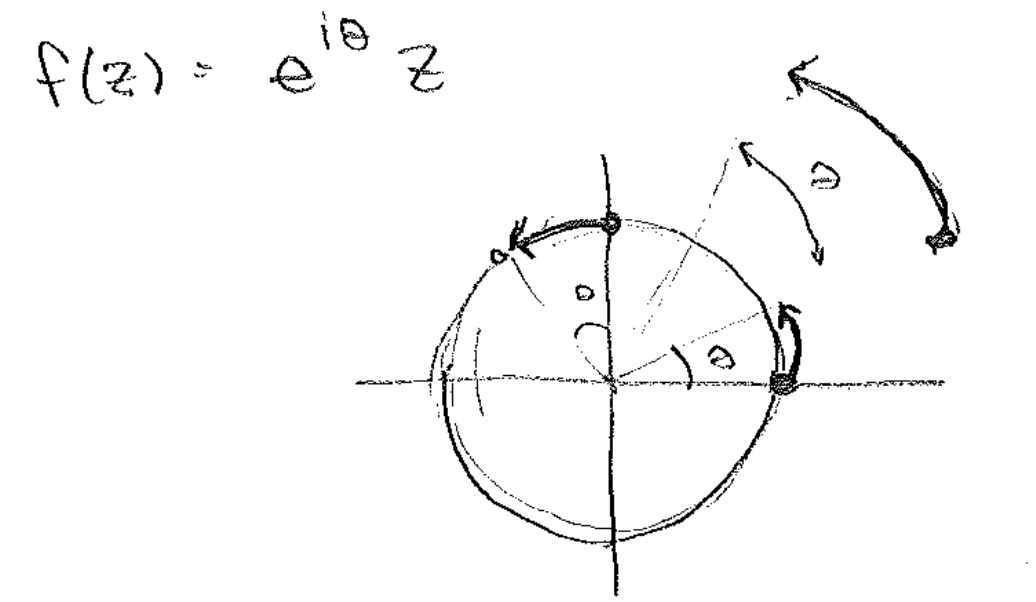
\includegraphics[width=.5\textwidth]{figures/lec13_map1.png}
\end{center}
\end{example}

\begin{exercise}
What happens to points under $f(z) = z+ z_0$?
\end{exercise}


\begin{example}
Now consider the simplest non-trivial polynomial, the function that squares its argument:
\begin{align}
	f(z) =  z^2 \ .
\end{align}
For a point $z = \rho e^{i\theta}$, $f(z)  = \rho^2 e^{2i\theta}$. This squares the modulus (length) of each point and rotates according to how much the point is already rotated relative to the positive real axis.
\begin{center}
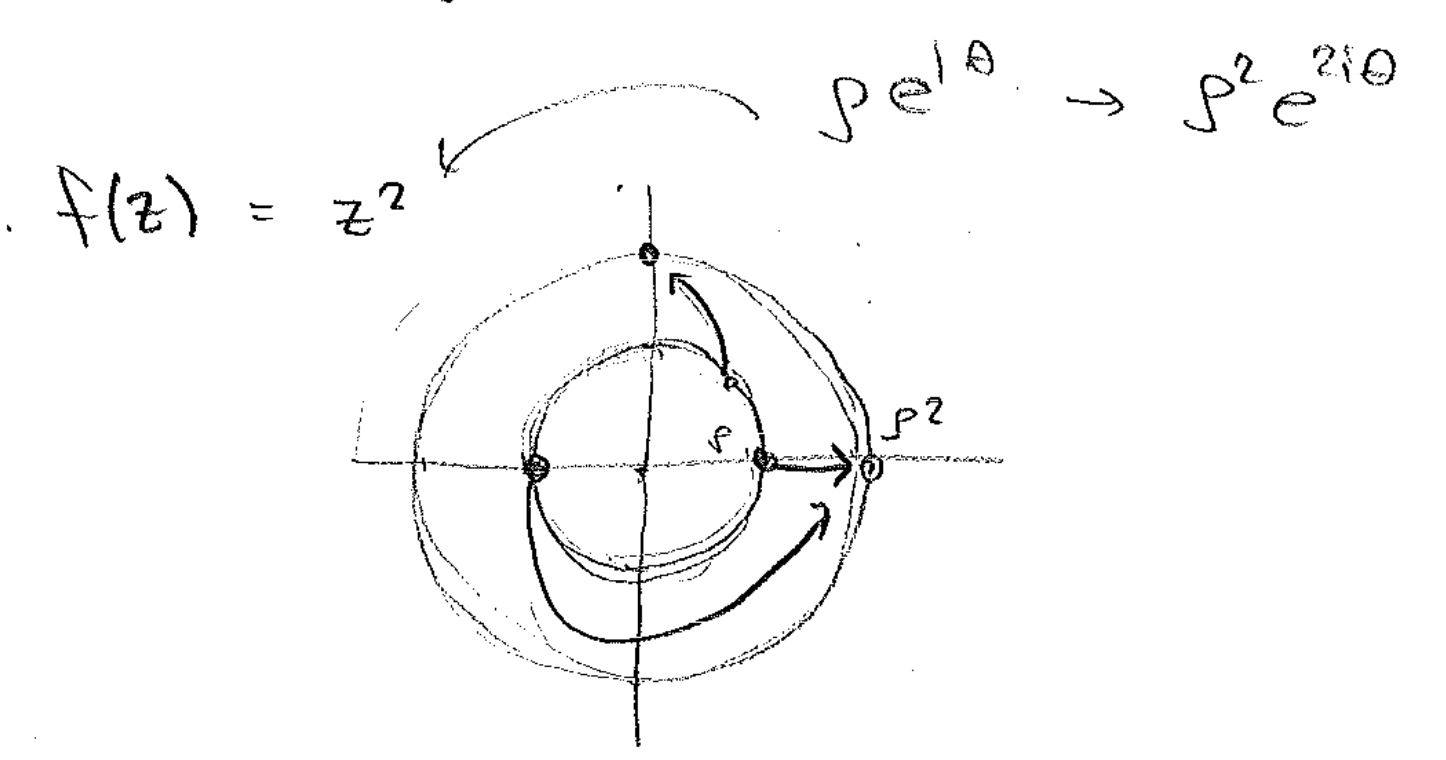
\includegraphics[width=.7\textwidth]{figures/lec13_map2.png}
\end{center}
Points that are inside the unit circle get pulled closer to the origin while points outside the unit circle are pushed away from the origin.  Points in the first quadrant (positive real and imaginary parts) are sent to points in the upper half plane (positive imaginary part).
\end{example}

\begin{exercise}
Show that under the map $f(z)=z^2$, a vertical line gets mapped onto a parabola:
\begin{center}
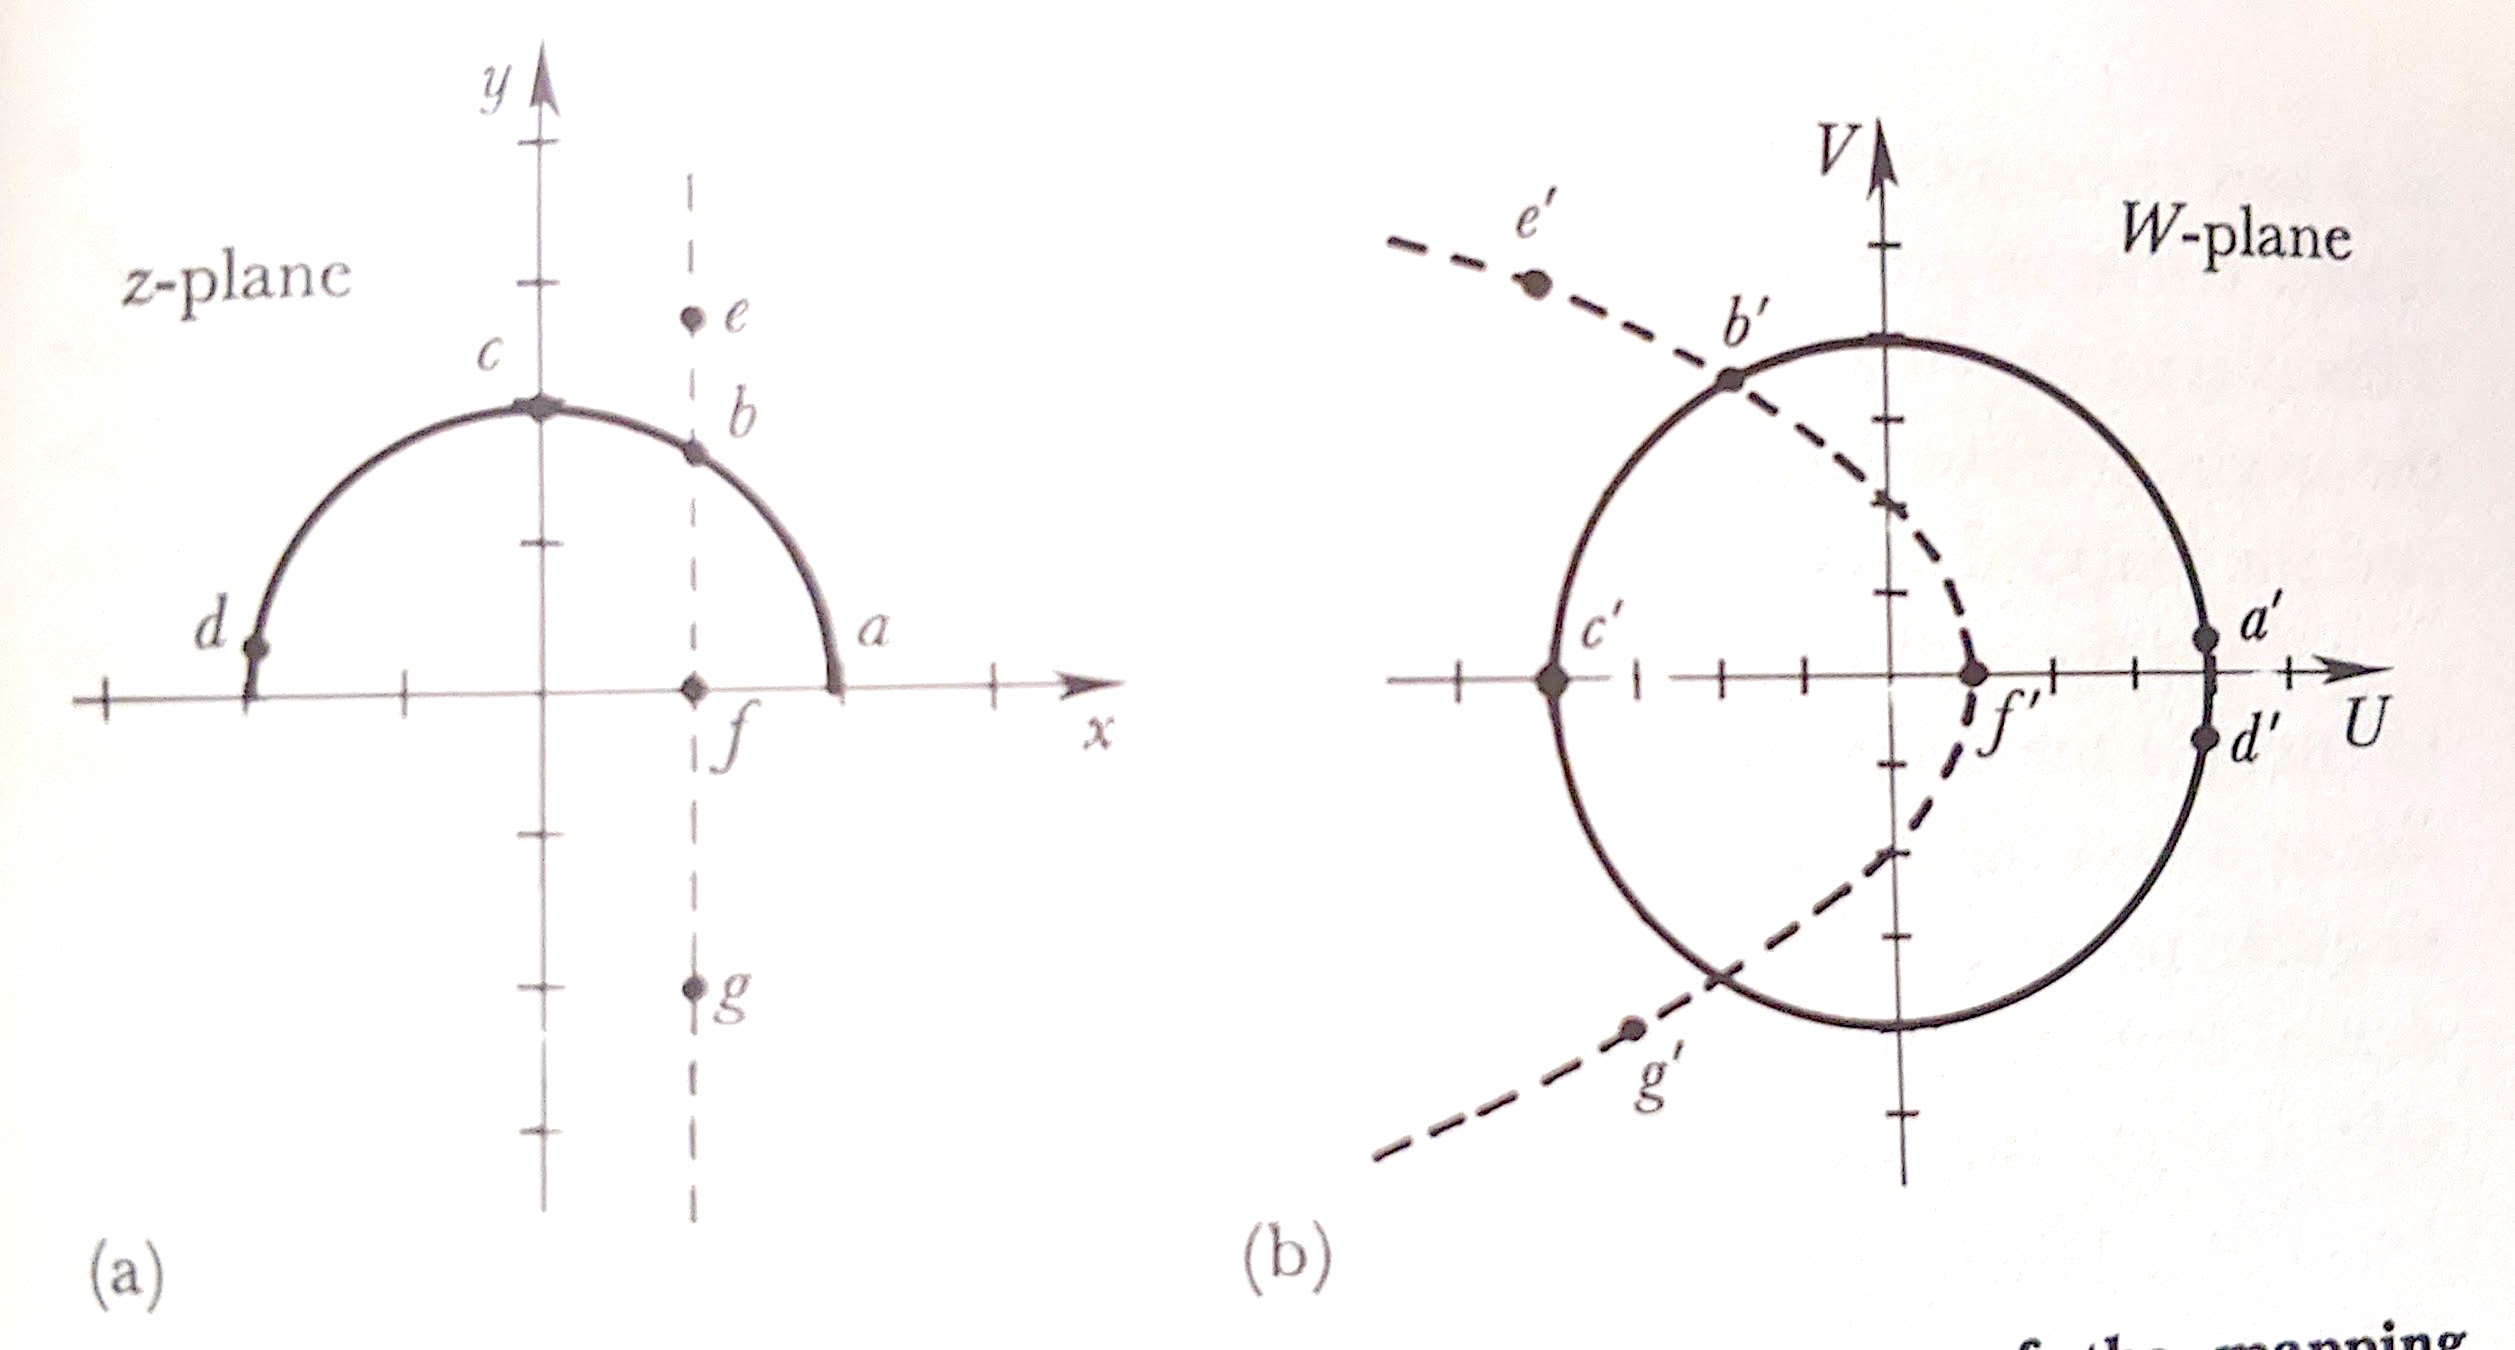
\includegraphics[width=.7\textwidth]{figures/lec13z2.jpg}
\end{center}
Figure from Matthews and Walker, points $a$, $b$, etc.\ are mapped onto $a'$, $b'$ etc. The $W$-plane corresponds to the image of the complex plan under $z^2$.
\end{exercise}

Now let's consider a curious case. What about the square root function?
\begin{align}
	f(z) = \sqrt{z} \ .
\end{align}
Something very weird happens here. Consider a closed path $\gamma(t) = e^{it}$ with path parameter $t \in [0,2\pi]$. This just means consider a bunch of points corresponding to $\gamma(t)$ with a bunch of values of $t$ in the specified range. Clearly this corresponds to a circle. However, when we put those points through the square root function, these only map onto \emph{half} of the circle. 
\begin{center}
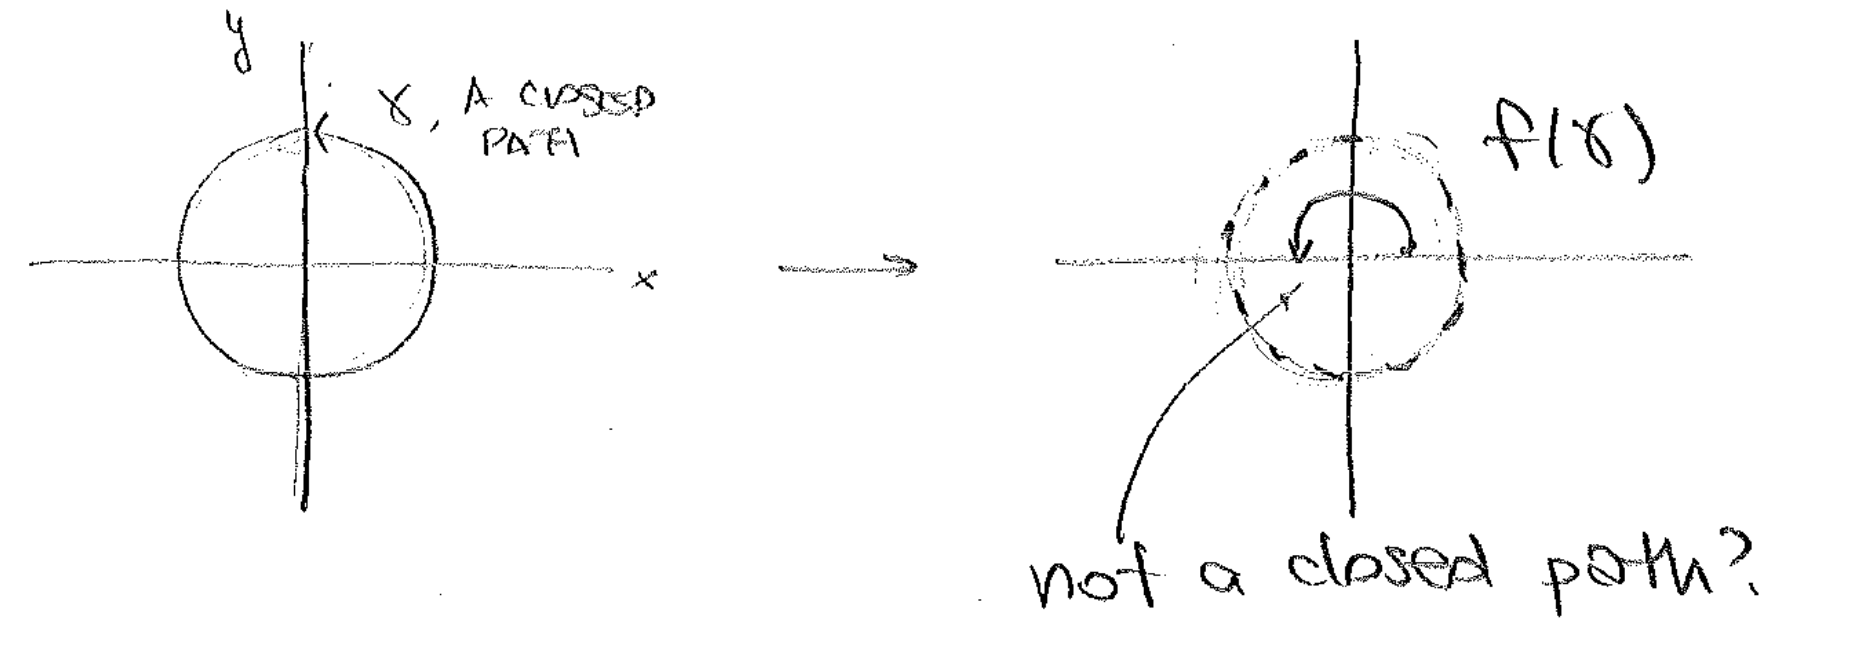
\includegraphics[width=\textwidth]{figures/lec13_map3.png}
\end{center}
The technical fact that this happens is not surprising at all, you can see that $f(\gamma(t)) = e^{it/2}$ which only spans the upper half circle. But a deeper question bubbles to the surface: if we're thinking about complex functions as maps of the complex plane to itself, what does it mean that $f(z) = \sqrt{z}$ appears to have `lost' the entire lower half of $\mathbbm{C}$? Or more strangely, how is it that a \emph{closed path} has been mapped to an \emph{open path} with endpoints?

It's clear that if we wanted to reach the \emph{lower} half plane in the iamage, we'd need $\theta \in [0, 4\pi]$. Algebraically that means that $f(\gamma(t)) = e^{it/2}$ covers the entire complex plane \emph{only} if we allow angles from 0 to $4\pi$
\footnote{You may be familiar with another case where `rotating by $2\pi$' only takes you halfway---spinors in relativistic quantum mechanics. You should know that the `double cover' nature of the spinor is (to the best of my view) independent of the present discussion of Riemann sheets. That double cover has to do with the universal cover of the Poincar\'e group. I refer to the literature on the Wigner theorem, see e.g.\ volume 1 of Weinberg's \emph{Quantum Theory of Fields}. For an unrelated cute spinor paper, see \url{https://www.jstor.org/stable/2318771}.}. In some sense, this is totally ridiculous, since $\rho e^{i\theta} \equiv \rho e^{i(\theta+2\pi)}$. I put that third bar on the equal sign because they're supposed to be \emph{that} equal.

If, say, $z_1=e^{i\pi/3}$ and $ z_2 e^{7i\pi/3}$ are supposed to be the \emph{same} point, $z_1\equiv z_2$, how is it that $f(z_1) = e^{i\pi/6}$ and $f(z_2) = e^{7i\pi/6}$ so that $f(z_1)\neq f(z_2)$? Stated differently, functions are supposed to be single valued. It appears that $f(z)=\sqrt{z}$ is \emph{multivalued} since the same point $z_1=z_2$ is mapped onto two different points. One way to do this is to \emph{define} additional structure and extend the domain (pre-image) of $f$. In order to do this, we take \emph{two} copies of the complex plane and stitch them together:
\begin{center}
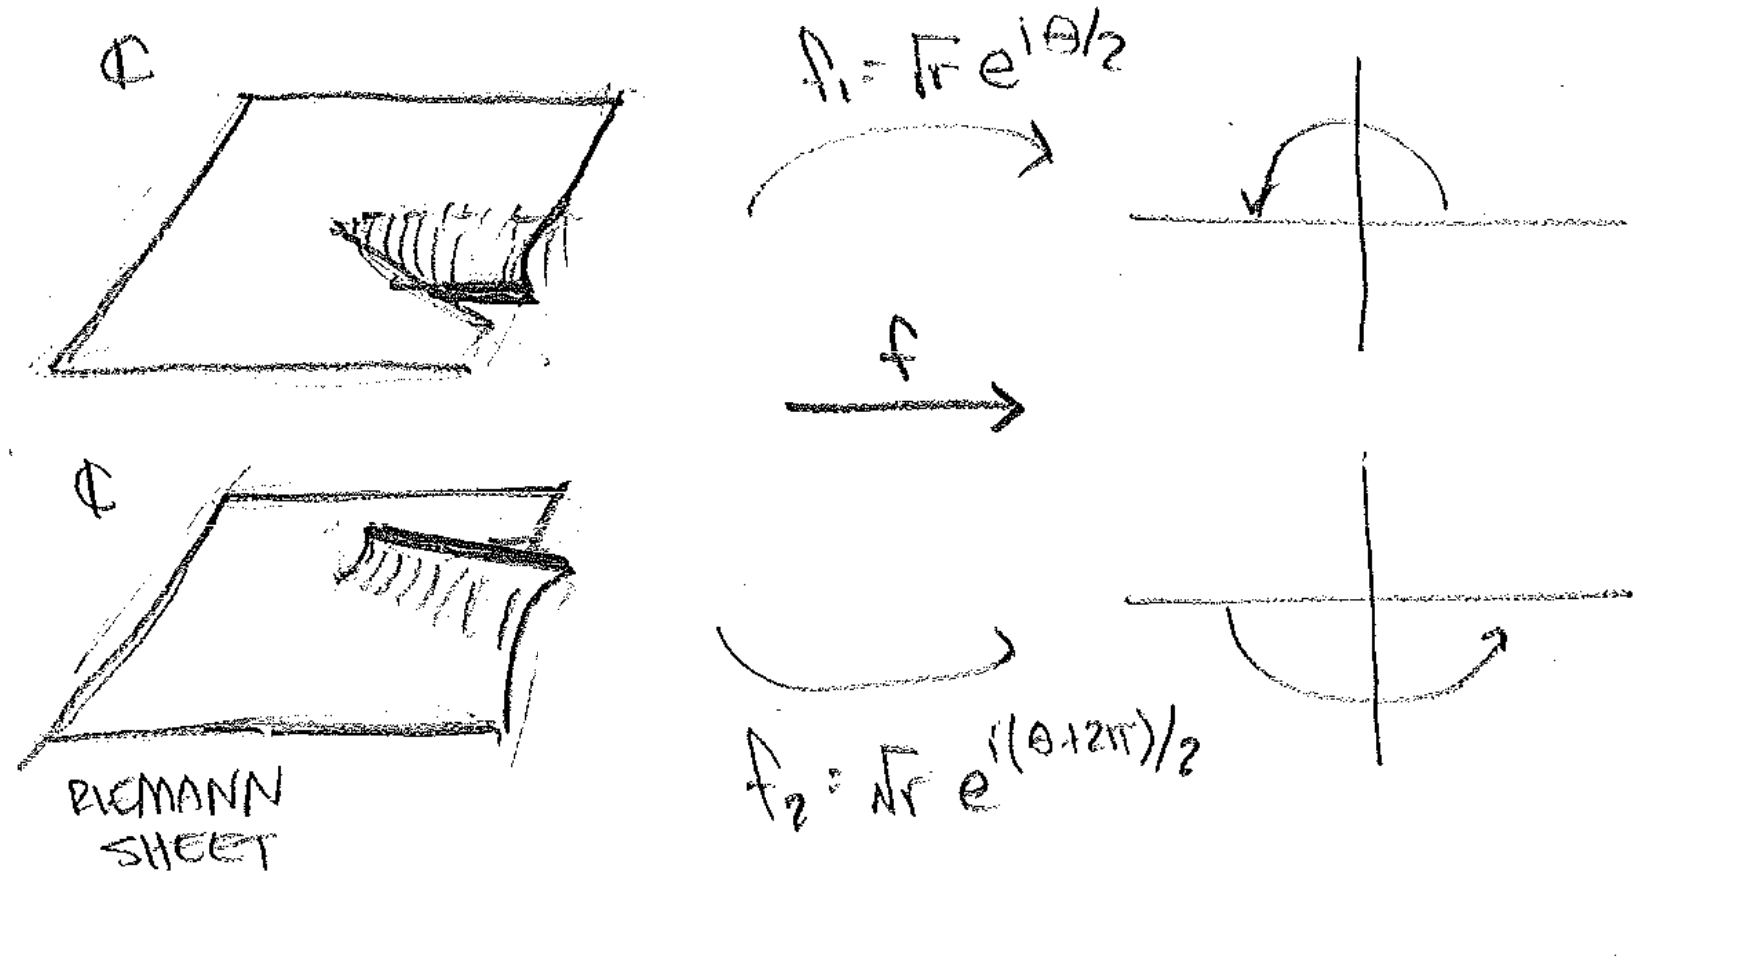
\includegraphics[width=.8\textwidth]{figures/lec13_map4.png}
\end{center}
Each copy of the complex plane is called a \textbf{Riemann sheet}. We `glue' these sheets together by defining that $\rho e^{i(\theta+2\pi)}$ of one sheet maps onto $\rho e^{i\theta}$ of the other sheet. Implicitly this chooses the positive real axis as a place where we \emph{cut} each sheet and glue them together. We call this a \textbf{branch cut}. One could, of course, have chosen the domain of each sheet to be any interval, say $\theta \in [-\pi,\pi]$ and picked a different branch cut ($\theta_\text{branch} = \pi$). 
\begin{exercise}
Is $f(z)=\sqrt{z}$ analytic on the extended complex plane (two Riemann sheets glued together at, say, $\theta=2\pi$)?
\end{exercise}
Take a moment to ponder the above exercise. As you may suspect, the relevant question isn't whether a function $f(z)$ `is analytic,' but rather \emph{where} is that function analytic? Is it analytic (differentiable) anywhere? Sure---when stay within one Riemann sheet, say $\theta\in (0,2\pi)$ and staying away from the boundary, $f(z)=\sqrt{z}$ is perfectly differentiable. Further, there's nothing special about the branch cut---we could have placed it anywhere. Thus it doesn't seem like there's \emph{any} place at which $f(z)$ is \emph{not} analytic. 

This should make sense: analyticity is about whether a function is differentiable at a given point. This is inherently a \emph{local} notion. The misbehavior of $f(z)=\sqrt{z}$---the necessity of Riemann sheets and a branch cut---are \emph{global} issues when we try to explore the \emph{whole} space. The interplay between local properties (like derivatives and Taylor expansions) and global properties (like integrals over a closed surface or topology) is a critical theme in mathematical physics. The function $f(z) = \sqrt{z}$ is analytic everywhere, but that doesn't mean we don't have to be careful. One of the lessons from this section is that the existence of a branch cut can be critically important if you happen to take trajectories that are \emph{loops} in the complex plane. For those who know where this is going: whenever there are branch cuts, you have to be careful with your contour integrals. This typically happens whenever you have a function that is not some series of integer powers of $z$.

As a final example, let's consider the complex logarithm. We'll use the notation of Byron and Fuller and write $\log$ to denote the complex natural logarithm and $\ln$ to denote the `usual' natural logarithm acting on real numbers. For $z=r e^{i\theta}$, the complex logarithm satisfies
\begin{align}
	\log z &= \ln r + i \theta
	\\
	\log(z_1z_2)
	&=\ln(r_1r_2) + i (\theta_1+\theta_2)
	= \log z_1 + \log z_2 \ .
\end{align}
\begin{example}
What does the domain of the complex logarithm look like? As a function, $f(z) = u(z) + i v(z)$, we see that $v(z) = \theta$ and $v(z_1z_2)=\theta_1+\theta_2$. This means that if we take a trajectory that keeps going around the origin, $v(z)$ just keeps increasing\footnote{This is where you can start humming `stairway to heaven.'}. Each time you go around you must be on a new Riemann sheet. 
\end{example}
Rather than having an infinite number of Riemann sheets, an alternative way of thinking about this is to imagine an infinite number of equally valid `complex logarithm' functions labeled by $n$:
\begin{align}
	f_n(z) &= \ln r + i \theta + 2\pi n i \ .
\end{align}
\begin{center}
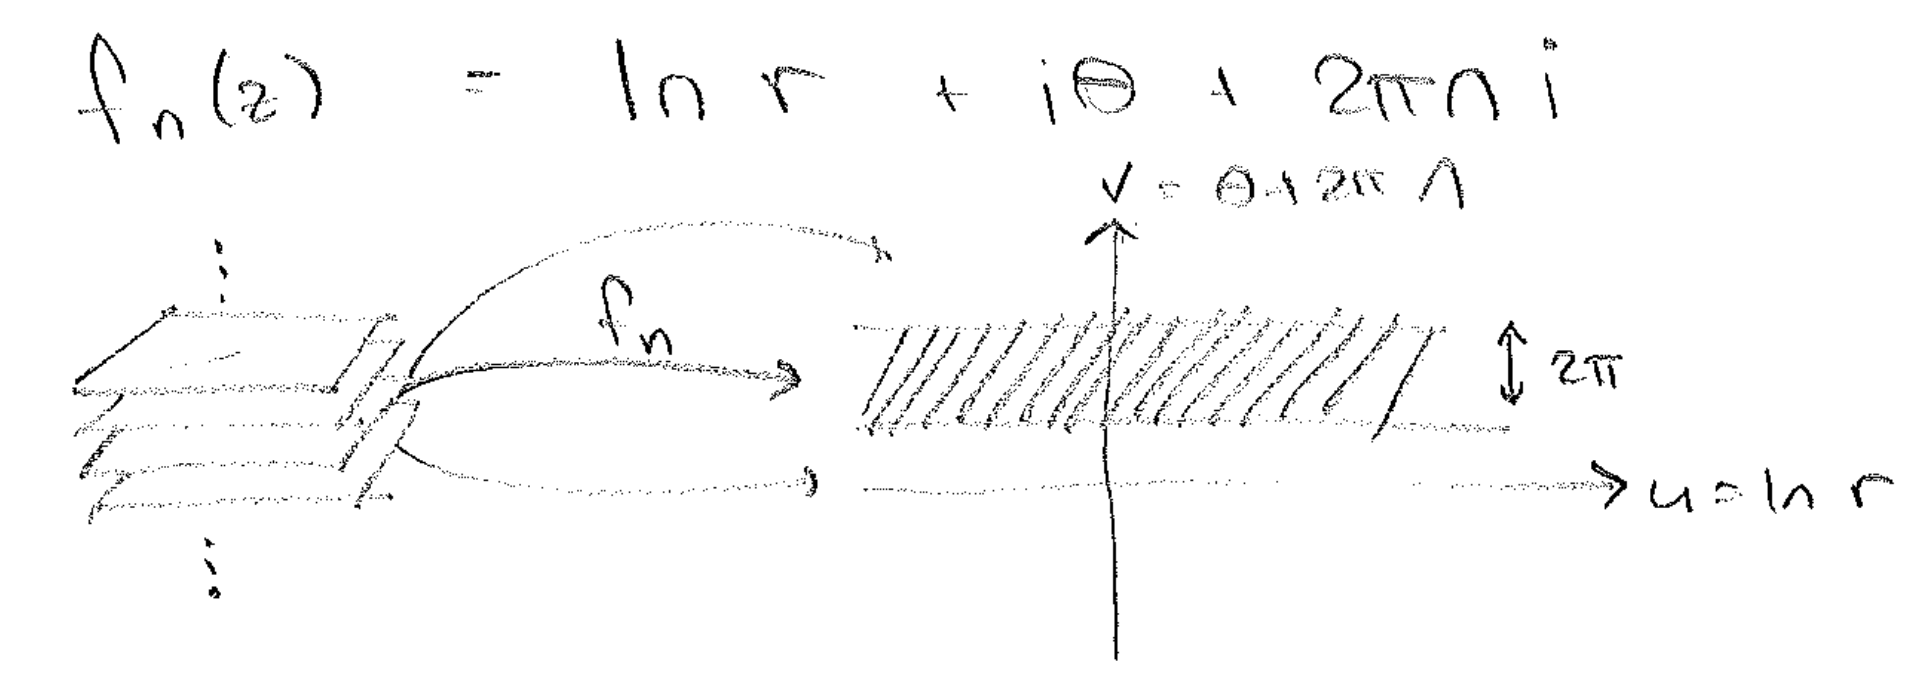
\includegraphics[width=\textwidth]{figures/lec13_map5.png}
\end{center}
The image of the $f_n(z)$ corresponds to a horizontal strip with $v\in \left(2\pi n, 2\pi(n_1)\right)$.
\begin{example}
Is the complex logarithm analytic? Everywhere but at $z=0$.
\end{example}
Let us end by repeating the main point of introducing branch cuts:
\begin{framed}
\begin{center}
Do not integrate across a branch cut!
\end{center}
\end{framed}

\subsection{Integration on the Complex Plane}
% StoGo 17.2.1

Let's now focus on integrating analytic functions. Oops, I just mis-spoke a bit there. What I meant to write was that we want to integrate functions in a region of $\mathbbm{C}$ where those functions are analytic. Rarely are functions simply `analytic' or `not-analytic.' The functions we care about will be analytic in most places, but non-analytic in others. 

When we integrate on the complex plane, $\mathbbm{C}$, we have to define a \textbf{contour}---this is just the curve, $C$, that we are integrating over. This is similar to doing a ``line integral'' in $\mathbbm{R}^2$: you are doing a `one-dimensional integral' over a two[ish]-dimensional space. An integral over the contour $C$ is:
\begin{align}
	\int_C dz\, f(z) &= 
	\int_C (dx + i dy) \ , \left[u(x,y)+ i v(x,y)\right]
	= 
	\int_C \left[u(x,y)dx - v(x,y)dy\right] 
	+ i \int_C \left[u(x,y)dy + v(x,y)dx\right] \ .
\end{align}
Written this way, we are simply doing calculus on $\mathbbm{R}^2$ and keeping track of funny factors of $i$. 
%
It may be helpful to remind ourselves what this means:
\begin{center}
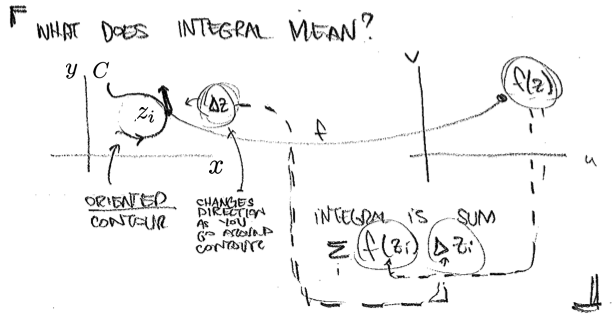
\includegraphics[width=\textwidth]{figures/Lec_2017_12_integral.png}
\end{center}
The integral along a curve can be thought of as two-dimensional version of a Riemann sum. Recall that the one-dimensional Riemann sum approximated the integral as a sum of terms $f(x_i)\Delta x$. In more than one dimension, the quantity $\Delta x$ is promoted to a `vector'\footnote{As I write this I feel sick to my stomach. In fact, $\Delta x$ is \emph{not} promoted to a `vector,' though it is promoted to something that points in a direction. More properly, it is a [differential] one-form which is more like an \emph{dual vector} in the sense referenced in Section~\ref{sec:analytic:geometric}.}. In other words, we may write
\begin{align}
	\int_C dz\, f(z) = \sum_i \Delta z_i \, f(z_i) \ ,
	\label{eq:complex:integral:Riemann}
\end{align}
where $\Delta z$ has a real and imaginary part: it \emph{points} to a direction in the complex plane. In the picture above, the left-hand side shows the curve $C$ on which we are integrating. Consider some point $z_i$ on the curve. That point is mapped by the function $f$ to a point $f(z_i) = u(z_i)+iv(z_i)$. At that point, the curve also has a differential element, $\Delta z_i$ which is tangent to the curve $C$ at point $z_0$ and has some fixed infinitesimal length for all $i$. The \emph{direction} of $\Delta z$ matters. It contributes to the overall phase of the term $\Delta z_i \, f(z_i)$.
\begin{example}
Consider the function $f(z) = z^2+i$.  Consider a specific point, $z_0 = 1+i$. If we consider different curves $C_i$ that pass through $z_0$, the integral $\int_{C_i}dz\,f(z)$ will have different contributions at $z_0$ depending on the \emph{direction of the curve} as it passes through $z_0$. To see this, consider the specific term in the sum \eqref{eq:complex:integral:Riemann} corresponding to $z_i = z_0$. If the curve $C$ happens to be moving in the positive vertical (pure imaginary) direction, then the contribution to the sum from this point is
\begin{align}
	\int_C dz\, f(z) = \cdots + i\Delta y\left[(1+i)^2 + i\right] + \cdots \ .
\end{align}
However, if the curve $C$ happens to be moving in the horizontal (pure real) direction, the contribution to the sum from this point is
\begin{align}
	\int_C dz\, f(z) = \cdots + \Delta x\left[(1+i)^2 + i\right] + \cdots \ .
\end{align}
\end{example}
\begin{exercise}\label{eq:fundamental:theorem:calculus}
Suppose $f$ is itself a derivative of an analytic function, $f(z)=dF(z)/dz$.
Convince yourself that if $C$ is a smooth connected path between two points $z_0$ and $z_N$, then the integral of $f(z)$ over $C$ is
\begin{align}
	\int_C dz\, f(z) &= F(z_N) - F(z_0) \ ,
\end{align}
as you would expect from real-number calculus.
% \footnote{By the way, this all a generalization of Stokes' theorem: the integral of the derivative of some function $f$ over some domain $D$ is simply the function evaluated on the boundary of the domain, $\partial D$. The $\partial D$ is notation for `boundary of $D$.' The fancy way to write this is
% \begin{align}
% 	\int_D df &= \int_{\partial D} f \ .
% \end{align}
% This statement holds for $f$ as a differential $n$-form (the generalization of a one-form and related to an $n$-index tensor) and $D$ is an $n$-dimensional domain. Even if you are not familiar with this nomenclature, please note the qualitative similarities with the integral of a derivative in 1D $\int dx\, (df/dx)$---which is simply the difference of $f$ at the endpoints of the domain, the integral of a curl in 2D---which is related to the `circulation' around the boundary of the 2D domain, and the integral of a divergence in 3D---which is simply related to the flux across the enclosing surface. Vector calculus isn't hard---it's just weird when we treat the 2D and 3D cases as different from the general $n$-dimensional case. 
% }.  
\end{exercise}


 

\subsection{Cauchy Integral Theorem}
% Cahill p. 160 for a sketch

As we may have referred to earlier---function that are analytic everywhere are too nice. Have you ever read a novel where everyone just got along nicely? Not very interesting. Complex functions are the same---it turns out that integrals of functions around closed curves in domains where they are analytic end up being zero. 

\subsubsection{Little tiny circles}

Let's show this starting from the simplest possible case. Consider a function $f$ that is analytic in some region $R\in \mathbbm C$. The boundary of this region is a curve $C = \partial R$. First consider the integral of $f$ around a small circle of radius $\varepsilon$ around some point $z_0$:
\begin{center}
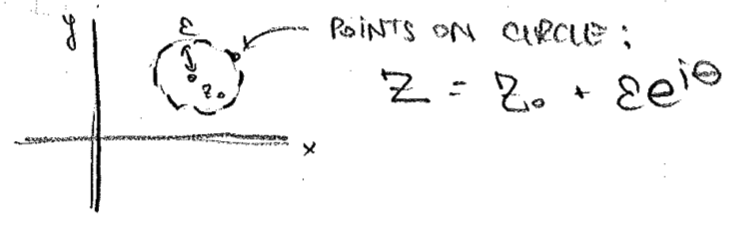
\includegraphics[width=.7\textwidth]{figures/Lec_2017_12_circle.png}
\end{center}
In other words, $C$ can be parameterized by the angle $\theta$. We can write points $z$ on the curve as
\begin{align}
	z(\theta) &= z_0 + \varepsilon e^{i\theta} 
	&
	dz &= i \varepsilon e^{i\theta} d\theta \ .
\end{align}
Then the integral around the little circle around $z_0$ is
\begin{align}
	\oint_C dz\, f(z) &= \int_0^{2\pi} i \varepsilon e^{i\theta} d\theta \, f\left( z_0 + \varepsilon e^{i\theta} \right) \ .
\end{align}
Now we observe that since $f$ is analytic, we can differentiate it---which means we can write it as a Taylor expansion:
\begin{align}
	f(z)
	 = f(z_0) + f'(z_0)(z-z_0) + \mathcal O(\varepsilon^2) \ ,
\end{align}
where we recognize that $z-z_0 = \varepsilon e^{i\theta}$. Plugging this in gives
\begin{align}
	\oint_C dz\, f(z) &= 
	\int_0^{2\pi} i \varepsilon e^{i\theta} d\theta \, f(z_0) 
	+
	\int_0^{2\pi} i \varepsilon^2 e^{2i\theta} d\theta \, f'(z_0) 
	+ \cdots
	\ .
\end{align}
Observe that the only $\theta$-dependence in the integrand shows up in factors of $e^{n i\theta}$ for positive integers $n$. However, we note that
\begin{align}
	\int_0^{2\pi} d\theta e^{in\theta} 
	= 
	\frac{1}{in} \left(e^{2\pi i n} - e^{0}\right)
	= 0 \ .
	\label{eq:complex:theta:integral:trivial}
\end{align}
What we find is that 
\begin{align}
	\oint_C dz\, f(z) &= 0
\end{align}
for the contour $C$ being a small circle around some arbitrary point $z_0$ inside the region $R$ in which $f$ is analytic. 
\begin{exercise}
Convince yourself that it didn't matter that $C$ is a small circle. It could have been any small shape. 
\end{exercise}
Notice that we did not rely on $\varepsilon\to 0$ in order to motivate this argument. The circle didn't actually have to be small. We used $\varepsilon\to 0$ to motivate the idea of truncating the Taylor series. But armed with \eqref{eq:complex:theta:integral:trivial}, we realize that \emph{every} term in the Taylor series will vanish, no matter how high the power since that simply corresponds to some larger positive integer $n$. At this point you should start to wonder whether there may be any loopholes in this argument.

\subsubsection{Finite regions}

Let's now prove a more general version of this known as the \textbf{Cauchy Integral Theorem}. If $f$ is analytic in a connected region $R \in \mathbbm{C}$ with some boundary $C = \partial R$ , then 
\begin{align}
	\oint_{C=\partial R} dz\, f(z) &= 0 \ ,
\end{align}
even if $R$ is some \emph{finite} region, not just some infinitesimally small circle. From the discussion of the case where $C$ is a little circle, you may have already guessed this. Let's show this more carefully. For any such region $R$, let's break it up into boxes:
\begin{center}
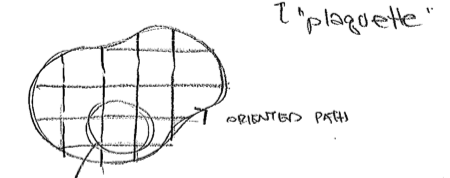
\includegraphics[width=.5\textwidth]{figures/Lec_2017_12_plaquette.png}
\end{center}
The boundary of a region $\partial R$ has some orientation. By convention a positive orientation corresponds to counterclockwise. Now that we've carved up the region $R$ into a grid like Manhattan\footnote{Search for `Manhattanhenge.' It has nothing to do with this course, but this is a photogenic consequence of the Manhattan grid.}, we integrate around the boundary of one of these \emph{plaquettes}:
\begin{center}
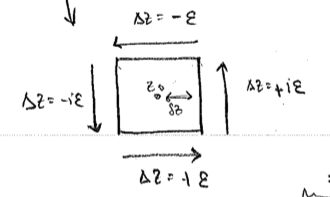
\includegraphics[width=.4\textwidth]{figures/Lec_2017_plaq_int.png}
\end{center}
We've assumed that each plaquette has characteristic size $\varepsilon$. Note that for each side of the plaquette the orientation of $\Delta z$ is different. Let $z_0$ correspond to the center of this plaquette. Since the function is analytic, we can write the function as a Taylor function around the plaquette:
\begin{align}
	f(z) = f(z_0) + f'(z_0) (z-z_0)^2 + \cdots
\end{align}
This means that we can approximate the integral around the square as
\begin{align}
	\oint_\text{plaquette} dz\,  f(z)
	&= 
	f(z_0)
	\left(
		\Delta z_1 + \Delta z_2 + \Delta z_3 + \Delta z_4
	\right)
	+ \cdots
\end{align}
where the $\Delta z_i$ are given in the figure above. It should be clear that the sum of the $\Delta z_i$ is zero since opposite sides give equal and opposite contributions. We have shown that to leading order the integral of an analytic function $f$ around a little box around it is zero---not too surprising given our previous result for integrating around a little circle. 
\begin{exercise}
What about the next-to-leading order contribution\footnote{Life advice: ``What about the next-to-leading order contribution'' is a good question to ask whenever you have shown that the leading order contribution is zero.}? Show that the next-to-leading order contribution, which goes like $\sum_i f'(z_0)\delta z_i \Delta z_i$ vanishes. Here the $\delta z_i$ is the separation from $z_0$ to the $i^\text{th}$ side, as shown in the figure above. 
% \begin{align}
% 	\left[
% 	\left(\frac{\varepsilon}{2}\right)
% 	(i\varepsilon)
% 	+
% 	\left(\frac{i\varepsilon}{2}\right)
% 	(-\varepsilon)
% 	+
% 	\left(-\frac{\varepsilon}{2}\right)
% 	(-i\varepsilon)
% 	+
% 	\left(-\frac{i\varepsilon}{2}\right)
% 	(\varepsilon)
% 	\right] = 0 \ .
% \end{align}
\end{exercise}
The above statement is true about each plaquette. However, note that when we piece the plaquettes together, the sum of the integrals around each little boundary corresponds to the integral around the boundary of the combined region:
\begin{center}
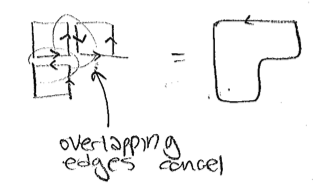
\includegraphics[width=.4\textwidth]{figures/Lec_2017_plaqses.png}
\end{center}
One can see that neighboring boundaries have opposite orientations so that the integrals along those regions cancel. 
%
This means that the integral around a the boundary $C$ of finite region $R$ is equivalent to the sum of the integrals around the little plaquettes that tile that region:
\begin{align}
	\oint_C dz\, f(z) &= \sum_i \oint_{\text{plaquette}_i} dz\, f(z) = 0 \ .
\end{align}
Since the integral around the boundary of each plaquette is zero, the integral along $C$ is zero. This proves the Cauchy integral theorem, which may now be stated as follows:
\begin{quote}
Analytic functions are \emph{so} nice that they're boring.
\end{quote}
In other words, if a function $f$ is analytic in a connected region $R$ and you try to integrate over a closed path $C$ that is inside $R$, then the result is zero. 

\subsection{An alternative argument (optional)}

% \footnote{By the way, this all a generalization of Stokes' theorem: the integral of the derivative of some function $f$ over some domain $D$ is simply the function evaluated on the boundary of the domain, $\partial D$. The $\partial D$ is notation for `boundary of $D$.' The fancy way to write this is
% \begin{align}
% 	\int_D df &= \int_{\partial D} f \ .
% \end{align}
% This statement holds for $f$ as a differential $n$-form (the generalization of a one-form and related to an $n$-index tensor) and $D$ is an $n$-dimensional domain. Even if you are not familiar with this nomenclature, please note the qualitative similarities with the integral of a derivative in 1D $\int dx\, (df/dx)$---which is simply the difference of $f$ at the endpoints of the domain, the integral of a curl in 2D---which is related to the `circulation' around the boundary of the 2D domain, and the integral of a divergence in 3D---which is simply related to the flux across the enclosing surface. Vector calculus isn't hard---it's just weird when we treat the 2D and 3D cases as different from the general $n$-dimensional case. 
% }.  

For those who are mathematically inclined, here's a geometrically-motivated argument for Cauchy's integral theorem. Consider two points $z_1$ and $z_2$ in a connected region $R$ where a function $f$ is analytic. Now consider any path $C_1$ that connects $z_1$ to $z_2$ and any other path $C_2$ that connects $z_2$ to $z_1$. The orientation matters.
\begin{center}
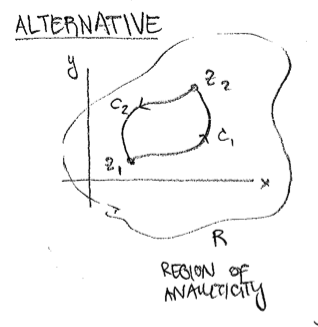
\includegraphics[width=.5\textwidth]{figures/Lec_2017_paths.png}
\end{center}
In the region of analyticity, a function $f(z)$ has an anti-derivative $F(z)$ such that $f(z) = dF(z)/dz$, recall Exercise~\ref{eq:fundamental:theorem:calculus}. Then we know that
\begin{align}
	\int_{C_1} dz\, f(z) &= F(z_2) - F(z_1)
	&
	\int_{C_2} dz\, f(z) &= F(z_1) - F(z_2) \ .
\end{align}
We deduce that the integral of the combined path $C=C_1+C_2$ is zero. The above argument is true without having to specify what $F(z)$ is and for \emph{any} paths $C_1$ and $C_2$ that share common endpoints. We thus prove Cauchy's Integral Theorem.

\paragraph{Commentary}
This argument is highlights a general idea in differential geometry, which is the generalized Stokes' theorem. In words, one can state this as:
\begin{quote}
The integral of the derivative of some function $f$ over some domain $D$ is simply the function evaluated on the boundary of the domain, $\partial D$. The $\partial D$ is notation for `boundary of $D$.'
\end{quote}
Technically it is relevant for the domain $D$ to be sufficiently \emph{nice}; this includes the domain being connected and having a reasonable boundary. Note that the boundary $\partial D$ is always oriented---when we integrate over an interval $[a,b]\in \mathbbm{R}$, the overall sign depends on which boundary is `on top' of the integral and which is `on the bottom.' In other words, it matters if we integrate over $[a,b]$ or $[b,a]$. 

We write formally as follows:
\begin{align}
	\int_D df &= \int_{\partial D} f \ .
\end{align}
Here the domain $D$ is an $n$-dimensional space and $df$ is called a \emph{differential} $n$-\emph{form}. From the name you should guess that it is related to the idea of a \emph{one-form} as a dual vector; see the optional discussion in Section~\ref{sec:analytic:geometric}.  This is a type of tensor with $n$ indices that is contracted with the `volume form' of the $n$-dimensional space. Formally it looks like this:
\begin{align}
	df &= (\partial_{\mu_1} f_{\mu_2\cdots \mu_n}) \; dx^{\mu_1}\wedge dx^{\mu_2}\wedge\cdots\wedge dx^{\mu_n} \ .
	\label{eq:Stokes}
\end{align}
The quantity $dx^{\mu_1}\wedge\cdots\wedge dx^{\mu_n}$ is the volume form and is an \emph{oriented} $n$-dimensional differential volume element. The funny wedge symbols ($\wedge$) represent an antisymmetric tensor product. This should not be so surprising: recall that the vector triple product $\vec{v}\cdot\left(\vec{w}\times\vec{u}\right)$ is a totally antisymmetric combination of vectors that produces the volume of the parallelogram with edges corresponding to the three vectors $\vec{v}$, $\vec{w}$, $\vec{u}$. This is precisely $\vec{v}\wedge\vec{w}\wedge\vec{u}$. The $n$-dimensional wedge product generalizes this notion to $n$-dimensional volumes. 

On the right-hand side of \eqref{eq:Stokes} is an integral over the \emph{boundary} of $D$. This is an oriented $(n-1)$-dimensional space. The integrand is the differential $(n-1)$-form. We thus see that the integral of $df$ over $D$ is related to a lower-dimensional integral of its primitive, $f$, on the boundary of $D$. 

Stokes' theorem is the underpinning of everything you've seen in vector calculus. In one dimension:
\begin{align}
	\int_a^b dx\, \frac{df(x)}{dx} = \int_{f(a)}^{f(b)} df = f(b)-f(a) \ .
\end{align}
In two dimensions, when you have a vector field $\vec{f}(x)$, the appropriate derivative (and the one that pops out of differential form notation) is the curl, $\nabla\times \vec{f}(x)$. This becomes an integral with respect to the differential surface element $d\hat{S} = \hat{\vec{n}} dS$, which may be chosen to be oriented in the $z$-direction perpendicular to the plane\footnote{Alternatively, $\hat{\vec{n}}$ is the unit normal of the 2D curved surface in a 3D space.}. Then we have the usual  Green's theorem:
\begin{align}
	\int_S dS\, \hat{\vec{n}}\cdot \left(\nabla\times \vec{f}(x)\right) 
	=
	\oint_{C=\partial S} \vec{f}(x)\cdot d\vec{x} 
	\ ,
\end{align}
where $d\vec{x}$ is a differential line element along the oriented curve $C$ that is the boundary of the integration region $S$. Finally, the divergence theorem in 3D relates the divergence of a vector field to its value on the surface:
\begin{align}
	\int_V dV \, \nabla\cdot \vec{f}(x)
	=
	\int_{S=\partial V} dS \, \hat{\vec{n}} \cdot \vec{f}(x) \ ,
\end{align}
where $\hat{\vec{n}}$ is the unit normal vector at each point on the surface $S$ bounding the volume $V$. These three versions of the `fundamental theorem of calculus' all look tantalizingly similar---and here we see that in fact, they're all manifestations of the general Stokes' theorem. 

Observe that the `boundary of a boundary' is nothing. If you have a disc, the boundary is a circle. The circle itself has no endpoints---in contrast to an interval. We can start to see some of the neat features of differential geometry when we look at Stokes' theorem, \eqref{eq:Stokes}, from this perspective. Indeed, one can read Stokes' theorem as a relation between the differential operator $d$ acting on an integrand and the `boundary operator' $\partial$  acting on the space. The `boundary of a boundary = 0' mantra can be loosely translated into `derivative of a derivative' is zero; where we are not being technically rigorous at all. You've already seen variants of this in vector calculus:
\begin{align}
	\nabla\times \nabla f(x) &= 0
	&
	\nabla \cdot \nabla\times \vec{f}(x) &=0 \ ,
\end{align}
and so forth. I used to think vector calculus was very challenging because there seemed to be so many different rules for how to differentiate and integrate. It turns out that differential geometry unifies this nicely into a general mathematical structure that, when applied to specific dimensions of space, produce all of the funny things you learn in undergraduate electrodynamics. It should not surprise you that this mathematical structure has a lot to say about the structure of theories like electrodynamics and gravity\footnote{One of my favorite introductions: \url{https://arxiv.org/abs/hep-th/0611201v1}.}.
\begin{exercise}
To see how this structure shows up in a simple physical system, look up Montgomery's treatment of the Falling Cat Problem. Similarly, Shapere and Wilczek's treatment of swimming animals at low Reynolds number. Wilczek famously won the Nobel prize for his contributions to the gauge theory of the strong nuclear force; a theory based on precisely this type of geometric structure we've discussed here. A final reference is to look up the Parallel Parking Problem, which was a topic of discussion in the first version of this P231 class that I taught in 2016. In that problem, one asks how a car can move transversely given that its only degrees of freedom are to move forward/backward and to turn the steering wheel. For the next two years students raised concerns that this class was hopelessly mathematical---so now here we are at the tail end of an exercise with no specific directions in an optional section of the lecture notes.
\end{exercise}

\subsection{Cauchy's Integral Formula}

Cauchy's Theorem tells us that integrating functions over domains where they are analytic is boring. Cauchy's Integral Formula\footnote{At this point you wonder: how is it that Cauchy got his name on everything in this business?} is the first step to something that is decidedly \emph{not} boring. The formula applies to a function $f$ that is analytic in some connected domain and a path $C$ entirely contained in that domain:
\begin{align}
	f(z_0) &= \frac{1}{2\pi i} \oint_C dz \frac{f(z)}{(z-z_0)}  \ .
	\label{eq:cauchy:integral}
\end{align}
This is the statement that the value of some function at some point $z_0$ is related to an integral of the function around the point. In fact, maybe this shouldn't be so surprising: the right-hand side looks like some kind of average of the function in the neighborhood of the function. Given the relation between analytic functions and harmonic functions, this sounds plausible. On the right-hand side there's a factor of $[2\pi (z-z_0)]^{-1}$ which indeed looks like one is averaging over the circumference around the point $z_0$. The factor of $i$ is curious. Those who are familiar with all of this will notice the `famous' combination $(2\pi i)$.

Let is highlight that the integrand on the right-hand side is 
\begin{align}
	g(z) &= \frac{f(z)}{z-z_0} \ .
	\label{eq:g:z:cauchy:integral:theorem}
\end{align}
Unlike $f(z)$, $g(z)$ is absolutely \emph{not} analytic `everywhere' in the region that we're looking at. It is not analytic at $z=z_0$. What's the derivative of $g(z)$ at the singularity? Heck if I know\footnote{Is it infinity? I suppose, but the notion of infinity in complex space can be a little tricky. At any rate, usually `infinity' is not the kind of answer that inspires much confidence.}. This is important because it is our first example of a function that is analytic in a region up to a single point\footnote{%
%
One observant student said that it is not obvious that $g(z)$ is non-analytic at the singularity $z=z_0$. If we define analytic to mean that a function is independent of $z^*$, then it is indeed not clear why $g(z)$ is non-analytic at $z_0$. This ends up being a failure of that definition: the more constructive definition of analyticity is having a unique and well-defined derivative as defined by the limiting procedure, $$\lim_{\Delta z\to 0}[g(z+\Delta z)-g(z)]/\Delta z \ .$$ 
%
}; we say that the function $g(z)$ has a \textbf{pole} at $z=z_0$.

Since the integrand $g(z)$ has a pole, we probably shouldn't integrate over it. No problem, our integration contour $C$ away from $z_0$. However, $z_0$ still punctures our domain over which the integrand is analytic\footnote{We've given our domain a topology. This, by the way, perhaps the one of the lamest things you can give someone. Once when I was a child I was sad when my parents got me a pair of socks for my birthday. I'd have been even more disappointed with topology. At least the socks kept my feet warm.}. To see what this does, let's consider the integral on the right-hand side.
\begin{center}
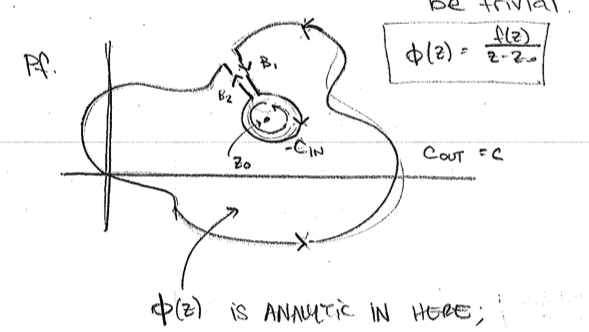
\includegraphics[width=.8\textwidth]{figures/Lec_2017_holes.png}
\end{center}
Let us call $C_\text{out}=C$, the original contour over which we're integrating. It is oriented counter clockwise by assumption. Because we're curious about the singularity at $z=z_0$, let's deform the contour by building a little bridge $B_1$ that heads towards $z_0$, then a little circle $-C_\text{in}$ that goes around the pole\footnote{Note the minus sign! We define $C_\text{in}$ to have positive/counter-clockwise orientation. In the picture above, we see that we traverse this little circle in the clockwise direction, so we put a minus sign on $C_\text{in}$.}, and then a little bridge $B_2$ that returns to $C_\text{out}$ where we originally left it. Clearly the integral over $B_1$ and $B_2$ cancel because
\begin{align}
	B_1 = -B_2
\end{align}
as paths. Note, however, that the region enclosed by the total curve $C_\text{out} +B_1-C_\text{in}+B_2$ is a region in which $g(x)$ is totally analytic. The $-C_\text{in}$ boundary separates the pole from the region enclosed\footnote{An engineer, a physicist, and a mathematician are tasked to optimize the amount of space surrounded by a finite length of fencing. The engineer builds a square pen since that makes it simple to construct. The physicist mumbles something about variational principles and builds a circle, stating that it optimizes the area enclosed for fixed perimeter. The mathematician takes the fence, throws away most of it, and then makes a tiny enclosure. The mathematician then carefully steps inside and says, ``I declare myself to be on the outside.''}. This means that Cauchy's Theorem holds. Because the bridge integrals over $B_1$ and $B_2$ cancel, the theorem tells us that
\begin{align}
	\oint_{C_\text{out}} dz\, g(z)
	-
	\oint_{C_\text{in}} dz\, g(z)
	= 0 \ ,
\end{align}\
where the minus sign came from $\oint_{-C_\text{in}} = - \oint_{C_\text{in}}$. The first term is precisely the right-hand side of \eqref{eq:cauchy:integral}. Apparently the second term is supposed to be $f(z_0)$. We can evaluate the second term along the contour by parameterizing $C_\text{in}$ as
\begin{align}
	C_\text{in}: \quad z(\theta) = z_0 + \varepsilon e^{i\theta} \ ,
\end{align}
which goes around $C_\text{in}$ for $\theta \in [0,2\pi]$. Now watch carefully. The relevant quantities in our integrand are:
\begin{align}
	dz &= i\varepsilon e^{i\theta} d\theta 
	&
	z-z_0 &= \varepsilon e^{i\theta} \ .
\end{align}
Now watch carefully: 
\begin{align}
	\oint_{C_\text{in}} dz\, g(z)
	=
	\oint_{C_\text{in}} dz\, \frac{f(z)}{z-z_0}
	= 
	i\int_0^{2\pi} d\theta f(z) 
	= 2\pi i f(z_0) \ . 
	\label{eq:cauchy:integral:theorem:step}
\end{align}
Note that once we wrote the integral with respect to $d\theta$, this is just an ordinary `real' integral where the integrand happens to have complex numbers in it. What is critical is that the powers of $e^{i\theta}$ canceled. Compare this to what happened in \eqref{eq:complex:theta:integral:trivial}, which was the analogous critical step for showing that the integral of analytic functions vanishes. In \eqref{eq:cauchy:integral:theorem:step} we ended up with \emph{no} factors of $e^{i\theta}$ so that the $d\theta$ integral ended up being non-zero. 
\begin{exercise}
Derive the last equality of \eqref{eq:cauchy:integral:theorem:step}:
\begin{align}
	i\int_0^{2\pi} d\theta f(z) 
	&= 2\pi i f(z_0) \ .
\end{align}
Why are we able to insert $f(z_0)$ in place of $f(z)$? Does this depend on the smallness of $\varepsilon$? (Answer: no.) {Hint}: $f(z)$ is analytic, which means it admits a Taylor expansion. Show that only the zeroth order term contributes, independently of how small $\varepsilon$ may be.
\end{exercise}

Putting this all together gives the desired result,
\begin{align}
	f(z_0) = \frac{1}{2\pi i}\oint_C dz\, \frac{f(z)}{z-z_0} \ .
	\label{eq:cauchy:integral:theorem}
\end{align}

The star of this discussion is not the analytic function $f(z)$; rather it is the analytic-up-to-a-pole function $g(z)$. Unlike our \emph{boring} scenario of functions that are analytic in a given domain, interesting stuff happens when our functions have singularities. We get to live dangerously and dance around theses singularities. In general, we will refer to singularities that go like $(z-z_0)^{-n}$ to be poles at $z=z_0$. The positive integer $n$ is called the order of the pole. The case $n=1$ is called a \textbf{simple pole}.

\subsection{From Taylor to Laurent}

Functions with poles are clearly not analytic \emph{everywhere}. However, they're pretty close to being analytic. They're analytic except for isolated poles. A function that is analytic up to poles is called \textbf{meromorphic}. If you're like me, you should classify these as \emph{nice, but not too nice} functions. They're just not-nice enough to be interesting. If you're keeping up with the `big picture,' you'll recall that the Fourier transform of a differential operator's Green's function  \eqref{eq:Greens:function:Fourier:transform:heuristic} appears to be in this class.

In a region where $f$ is analytic, differentiability meant that one could write a Taylor expansion: a series of terms that go like $(z-z_0)^n$ for positive integers $n$. When $f$ is merely \emph{meromorphic}, the Taylor expansion is generalized to a \textbf{Laurent expansion}:
\begin{align}
	f(z) = \sum_{n=-N}^\infty  a_n(z_0) (z-z_0)^n \ ,
\end{align}
where $N$ is the order of the pole at $z_0$ (if there is one). 

\subsection{The Residue Theorem: a first look}

Now we arrive at our mail tool. Suppose $f(z)$ is meromorphic in some region of the complex plane. In fact, suppose $f(z)$ has a simple pole at $z_0$; the function $g(z)$ in \eqref{eq:g:z:cauchy:integral:theorem} is a function precisely of this type. Consider the integral of $f(z)$ around a closed contour that goes around the pole once. For example, the pole is in some connected region $R$ and the contour is the boundary of this region, $C=\partial R$. Applying the Laurent expansion about $z_0$ for this meromorphic function $f$ gives
\begin{align}
	\oint_C dz\, f(z) &= \oint_C dz 
	\left[
	\sum_{n<0} a_n (z-z_0)^n + \sum_{n\geq 0} a_n (z-z_0)^n
	\right] \ .
\end{align}
All we have done is separated the positive-power terms of the Laurent expansion from the negative power terms. We know that the positive power terms integrate to zero because those terms are analytic in $R$. Thanks, Cauchy's Theorem.

What about the term with negative powers? Since we assumed that $z_0$ is a simple pole, we know that only the $a_{-1}$ term is non-zero in this Laurent expansion about $z_0$. That means that we can write the integral as
\begin{align}
	\oint_C dz\, f(z) &= 
	\oint_C dz \,
	\frac{a_{-1}}{z-z_0} 
	\ .
	\label{eq:residue:int:step:1}
\end{align}
The coefficient $a_{-1}$ of the Laurent expansion about a pole is called the \textbf{residue} of the function $f$ at the pole $z_0$. We will use the notation $\text{Res}_f(z_0)$. 


Now recall Cauchy's Integral Theorem. For the sake of clarity (I have used $f$ too many times), let us write the integral theorem with respect to an analytic-in-this-neighborhood function $h$:
\begin{align}
	\oint_C \frac{h(z)}{z-z_0} = {2\pi i} \, h(z_0) \ ,
\end{align}
we've gone ahead and re-arranged some terms. Comparing this to \eqref{eq:residue:int:step:1}, we may take $h(z) = a_{-1} = \text{Res}_f(z_0)$. This means that $h(z_0) = \text{Res}_f(z_0)$ so that we ultimately have
\begin{align}
	\oint_C dz\, f(z) &=  2\pi i  \, \text{Res}_f(z_0) \ .
\end{align}
We will generalize this shortly, but the main idea is in this simple example. If you can identify the $a_{-1}$ coefficient of a meromorphic function at its pole, then you can easily integrate the function around the pole. As long as there aren't any other poles in the neighborhood, it doesn't matter what your contour is as long as you are going around counter-clockwise and you go around exactly once.


% Lec 13

\subsection{The Residue Theorem: more carefully}

The residue theorem is our primary tool for calculating integrals on the complex plane. Let's see how it generalizes. Consider a meromorphic function $g(z)$ with two simple poles:
\begin{align}
	g(z) &= \frac{h(z)}{(z-z_1)(z-z_2)} 
	&
	h(z) \text{ analytic over }\mathbbm{C} \ .
\end{align}
The simple poles are located at $z=z_1$ and one at $z=z_2$. Consider a contour $C$ that encloses both poles. The integral of $g(z)$ along $C$ is simply $2\pi i$ times the sum of the residues of the two simple poles. This is easy to see from dividing $C$ into the sum of two paths:
\begin{center}
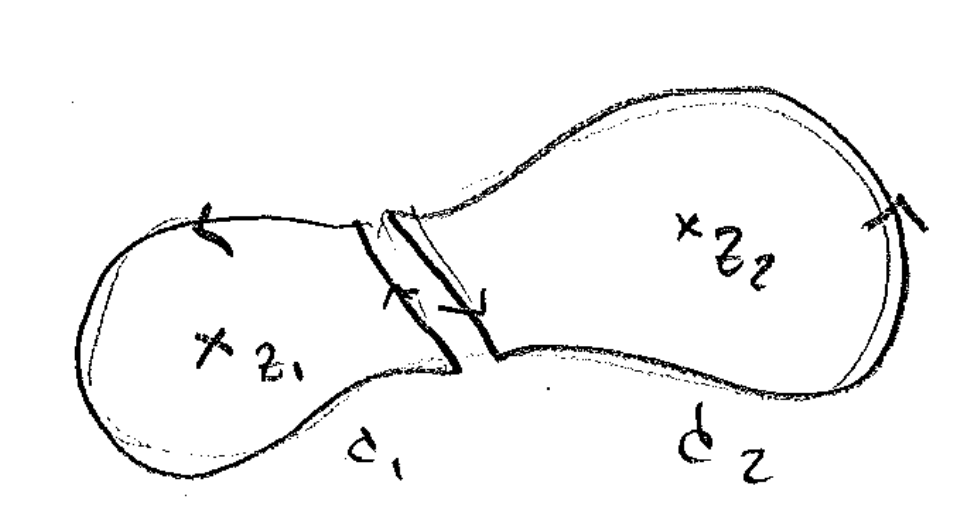
\includegraphics[width=.5\textwidth]{figures/Lec_2017_13_2poles.png}
\end{center}
Here $C_1$ is a closed contour that encloses $z_1$ but not $z_2$. Similarly, $C_2$ is a closed contour that encloses $z_2$ but not $z_1$. Observe that $C_1$ and $C_2$ overlap along a line that separates the two poles. Because both $C_1$ and $C_2$ are positively oriented, the integrals along this line cancel. From this it is clear that
\begin{align}
	\oint_C dz\, g(z) &=
	\oint_{C_1} dz\, g(z) 
	+
	\oint_{C_2} dz\, g(z)
	= 2\pi i\left(\text{Res}_f(z_1) + \text{Res}_f(z_2)\right) \ .
\end{align}
This gives a more general form of the residue theorem. The integral of a meromorphic function $f(z)$ around a closed contour $C$ that is the boundary of some region of the complex plane\footnote{Note that this means that $C$ is positively oriented and only circles around the region once.} is
\begin{align}
	\oint_C dz\, f(z) &= 2\pi i \sum_{i\in \text{poles}} \text{Res}_f(z_i) \ ,
\end{align}
where the sum is over the poles of $f$ at $z_i$ enclosed inside $C$.
\begin{exercise}
How would the residue theorem change if the contour $C$ were oriented in the opposite direction? What if the contour circled the poles multiple times? What if the contour circled some poles some number of times, and other poles a different number of times?
\end{exercise}


\subsection{Non-simple poles (a case study in being careful)}

So far we've focused only on meromorphic functions that have \emph{simple} poles. What about higher order singularities? Here's a tangible example:
\begin{align}
	\oint_C dz \, f(z) = ?
	&&
	f(z) &= \frac{1}{(z-2i)^2} \ ,
	\label{eq:non-simple:pole:example}
\end{align}
where $C$ is a positively oriented contour that circles the second-order pole $z_0 = 2i$. Because $f(z)$ has no simple pole at $z_0$, it looks like there's no contribution to the integral. To check this, we recall Cauchy's integral formula, \eqref{eq:cauchy:integral:theorem:step}. The reason why simple poles contributed to the contour integral is the observation that for an integer,  $n$, the integral of $e^{in\theta}d\theta$ behaves as follows: 
\begin{align}
	\int_0^{2\pi}d\theta\, e^{in\theta} 
	&=
	\begin{cases}
	0 & \text{\quad if } n\neq 0
	\\
	2\pi  & \text{\quad if } n= 0
	\end{cases} \ .
\end{align}
Following the same in the previous sub-sections, the integral in \eqref{eq:non-simple:pole:example} about a contour $C$ that circles $z_0=2i$ once is equivalent to the integral over smaller contour $C'$ that is a small circle that surrounds $z_0$. Parameterize $C'$ by the angular variable:
\begin{align}
	z(\theta) &= z_0 + \varepsilon e^{i\theta} & dz &= i\varepsilon e^{i\theta} \, d\theta \ .
\end{align}
Then the integral is:
\begin{align}
	\oint_C dz\, f(z) 
	= 
	\oint_{C'} dz\, f(z) 
	= 
	\int_0^{2\pi} i\varepsilon e^{i\theta} d\theta\, 
	\frac{1}{\varepsilon^2 e^{2i\theta}} 
	=
	\frac{i}{\varepsilon}
	\int_0^{2\pi} d\theta\, 
	e^{-i\theta}
	= 0 \ .
	\label{eq:non-simple:pole:eg:zero}
\end{align}
So this is all consistent with the mantra of \emph{find the $a_{-1}$ coefficient of the Laurent expansion, that's the residue}. 

We should be careful, though. If we're too slick we can convince ourselves of wrong things. For example, suppose we wanted to generalize \eqref{eq:non-simple:pole:example} by changing the numerator of $f(x)$:
\begin{align}
	\oint_C dz \, f(z) = ?
	&&
	f(z) &= \frac{h(z)}{(z-2i)^2} \ ,
	\label{eq:non-simple:pole:example:hz}
\end{align}
where $h(z)$ is an analytic function. For the sake of argument, let's assume that $h(z)/(z-2i)^2$ has been simplified so that there are no common factors between the numerator and denominator\footnote{For example, if $h(z)=(z-2i)$ then clearly $f(z)$ has a simple pole at $z_0=2i$ so the integral picks up a non-zero residue.}. One might think that when we shrink the contour from $C$ to $C'$, we can approximate $h(z)= h(z_0)$ so that
\begin{align}
	\oint_{C'}dz\, f(z)
	&=
	\oint_{C'} i\varepsilon e^{i\theta}d\theta\, 
	\frac{h(z_0)}{\left(z-2i\right)^2}
	=
	\frac{i}{\varepsilon}h(z_0)
	\int_0^{2\pi} d\theta\, 
	e^{-i\theta}
	= 0\,?
\end{align}
In general, this argument is \emph{wrong}. It is wrong even though the \eqref{eq:non-simple:pole:eg:zero} happens to be true. 
\begin{exercise}
Can you spot the incorrect assumption?
\end{exercise}
The incorrect assumption is that we could approximate $h(z) = h(z_0)$ because the little circle $C'$ is always close to $z_0$. The intuition is fine, but we weren't careful enough: even though $h(z)$ is analytic everywhere, we should remember write a Taylor expansion:
\begin{align}
	h(z) = h(z_0) + h'(z_0)(z-z_0) + \cdots
\end{align}
Even if our intent is to only keep the first term, it's a good habit to remember that the Taylor expansion contains many terms. Let's see what happens: 
\begin{align}
	\oint_{C'}dz\, f(z)
	&=
	\oint_{C'} i\varepsilon e^{i\theta}d\theta\, 
	\frac{h(z_0)+ h'(z_0)(z-z_0) + \cdots}{\left(z-2i\right)^2}
	\\
	&
	=
	\frac{ih(z_0)}{\varepsilon}
	\int_0^{2\pi} d\theta\, 
	e^{-i\theta}
	+
	{ih'(z_0)}
	\int_0^{2\pi} d\theta
	+\cdots
	\label{eq:non-simple:pole:example:hz:punchline}
\end{align}
While the first term vanishes, the second term is clearly non-zero since it's a contour integral. Indeed, one ends up with
\begin{align}
	\oint_{C'}dz\, \frac{h(z)}{(z-2i)^2}
	= 2\pi i h'(z_0) \ ,
\end{align}
where evidently $\text{Res}_f(2i)=h'(2i)$ is the residue of $f(z)=h(z)/(z-2i)^2$ at $z_0=2i$. 
\begin{exercise}
Why don't higher order terms in \eqref{eq:non-simple:pole:example:hz:punchline} do not contribute to the contour integral.
\end{exercise}
The purpose of this example was to show that it can be a little tricky to identify the residue of a function by simply `looking at the denominator.' You will derive an explicit formula in your homework. Fortunately, we will rarely consider non-simple poles in this course. 

% Lec 14 2017

Let's go through a few examples. These are from the third edition of Boas, chapter 14.6. 

\begin{example}
Let $f(z)=\cot z$. Find the residue of $f$ at $z=0$. 

To solve this, we can write out the numerator and denominator of the cotangent:
\begin{align}
	\cot z &= \frac{\cos z}{\sin z}
	= \frac{1-z^2/2 + \cdots}{z - z^3/3!} \ .
\end{align}
From this we see that $z\to 0$ is indeed a simple pole, and one may write the residue as
\begin{align}
	\text{Res}_f(0) &= \lim_{z\to 0} z \frac{1}{z} = 1 \ .
\end{align}
\end{example}


\begin{example}\label{ex:cot:2:residue}
Let $f(z)=\cot^2 z$. Find the residue of $f$ at $z=0$. 

Writing out the numerator and denominator again:
\begin{align}
	\cot^2 z &= 
	= \frac{1-z^2 + \cdots}{z^2 - 2z^3/3! + \cdots} 
	\sim \frac{1}{z^2} + \mathcal O(1)
	\ .
\end{align}
From this we deduce that $\text{Res}_f(0) = 0$. 
\end{example}

\begin{exercise}
Why were we able to be slick in Example~\eqref{ex:cot:2:residue} after making a big deal about being careful in \eqref{eq:non-simple:pole:example:hz:punchline}?
\end{exercise}

\begin{exercise}
Let $f(z)=z\cot^2 z$. Find the residue of $f$ at $z=0$. 
\end{exercise}


\begin{exercise}
Let $f(z)$ be
\begin{align}
	f(z) &= \left(\sum_{n=0}^\infty c_n z^n\right)\cot^2 z
\end{align}
Show that the residue of $f$ at $z=0$ is $c_1$.
\end{exercise}


\subsection{The Killer App: Real Integrals}

The \emph{killer app}\footnote{This is an old phrase from the first dot-com bubble.} for complex contour integrals is to solve integrals along the \emph{real line}. It is often the case that some of the real functions that we would like to integrate happen to have poles in the complex plane. In this case, the integral along the real line can be completed into a closed contour $C$ in the complex plane. If we can separate the contribution of the real line from the rest of the contour, then we can use the residue theorem to do the integral without any of the hard work of, uh, integrating.

\begin{example}
Consider the real function
\begin{align}
	f(x) = \frac{1}{x^2 +1} \ .
\end{align}
Typically we care about real functions with real arguments. However, let's \emph{analytically continue} $f(x)$ into a meromorphic function $f(z)$
\begin{align}
	f(z) = \frac{1}{z^2+1} \ .
\end{align}
This is the (unique\footnote{The proof is left to you to derive or look up.}) complex function that is analytic and agrees with the original function on the real line. We immediately notice that $z^2+1 = (z+i)(z-i)$ so that $f(z)$ has simple poles at $z=\pm i$. Consider the following contour which includes the real interval $x\in [-R,R]$ as part of it:
\begin{center}
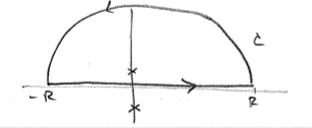
\includegraphics[width=.7\textwidth]{figures/Lec_2017_14_contour.png}
\end{center}
We will care about the limit $R\to \infty$ where the integral includes the entire real line.
Observe that the contour only encloses the pole at $z=i$. Let us integrate the function around $C$. From the residue theorem, we have
\begin{align}
	\oint_Cdz\, \frac{1}{(z+i)(z-i)} 
	= 2\pi i \text{Res}_f(i) 
	= \pi \ ,
\end{align}
where we've used $\text{Res}_f(i)=1/2i$. However, we can also write the integral as a sum of the real integral plus a counter-clockwise arc of radius $R$:
\begin{align}
	\oint_C dz\, f(z) = \int_{-R}^R dx\, f(x) 
	+ \int_0^\pi iR e^{i\theta} d\theta  \, f\left(Re^{i\theta}\right) \ .
\end{align}
where in the second term we've used the parameterization $z(\theta) = Re^{i\theta}$. Note that the first term on the right-hand side is the `ordinary' purely real integral. The second term behaves as follows:
\begin{align}
	\int_0^\pi iR e^{i\theta} d\theta  \, f\left(Re^{i\theta}\right)
	&= 
	\frac{Re^{i\theta}}{R^2 e^{2i\theta}+1} d\theta \ .
\end{align}
As we take the limit $R\to\infty$, the integral goes like $\sim 1/R \to 0$. Thus as long as we actually care about the integral along the entire real line, $R\to \infty$, we have
\begin{align}
	\oint_Cdz\, \frac{1}{(z+i)(z-i)}  
	= \pi 
	= \lim_{R\to\infty} \int_{-R}^R \frac{dx}{x^2+1} \ .
\end{align}
And so we find
\begin{align}
	\int_{-\infty}^\infty dx \, 
	\frac{dx}{x^2+1}
	= \pi \ .
\end{align}
This is an absolutely correct result about a \emph{real} integral that we sneakily derived without actually doing the integral. I assume one may check this by the appropriate trigonometric substitution\footnote{Just kidding, you can just check it on \emph{Mathematica}. You can even tell people that you did the trig substitution if it makes you feel better.} Observe that the critical step was that the curved part of the contour (the one that actually had imaginary parts) went to zero in a well defined limit. 
\end{example}
\begin{exercise}
What result do you get when you solve for the same integral of function $f(x)=(x^2+1)^{-1}$ over the real line, but this time you use the contour $C'$ that encircles the lower half of the complex plane?
\end{exercise}
Let's address the question of \textbf{analytic continuation}\footnote{See Appel section 5.3 for a more careful discussion.}. We started with a purely real function $f(x)$ and `generalized it' to a complex function $f(z)$ that happened to have poles in the complex plane. Because we used the residue theorem, the details of these poles (residue and whether they're enclosed by $C$) are critical for performing the integral. So a good question is: is the \emph{complex function} $f(z)$ even uniquely defined given the \emph{real} function $f(x)$?\footnote{My notation is a little glib and assumes the answer. If you want, you can write $f_\mathbbm{C}$ and $f_\mathbbm{R}$ to differentiate the two functions that are different in principle.}
\begin{center}
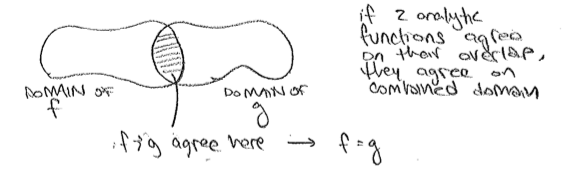
\includegraphics[width=.9\textwidth]{figures/Lec_2017_14_analytic_continuation.png}
\end{center}
There is a handy theorem that states that when two analytic functions agree on their domain of overlap, then they agree on their common domain. For \emph{meromorphic} functions, we can just imagine the domain where those singularities are not included. In our example above, $f(x)$ is analytic along the real line and $f(z)$ is a function that trivially (by construction) is analytic and matches $f(x)$ on the real line. Then the theorem says that $f(z)$ and $f(x)$ `agree' in the entire domain of analyticity; so one can \emph{analytically continue} $f(x)$ to the complex plane as long as one avoids any singularities.

The gist of the proof is that if two functions $f$ and  $g$ agree in some overlapping domain of analyticity, then their difference $h(z)\equiv f(z)-g(z)$ is also an analytic function in this domain. Analyticity means one has finite radius of convergence because it has a well defined Taylor expansion. One can then use this to argue that $h(z)$ can be defined beyond the overlapping domain. Continuity requires that $h(z)$ remains zero even outside the overlapping domain, which ensures that $f(z)=g(z)$. In other words, there is a unique analytic continuation of a function to a maximal domain of analyticity.

There's another effect you may wonder about. Are there some `edge' effects from the corner of the contour?
\begin{center}
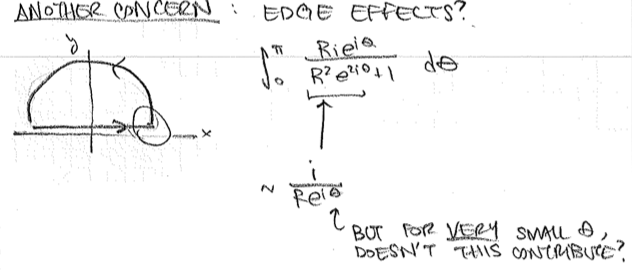
\includegraphics[width=.9\textwidth]{figures/Lec_2017_corner.png}
\end{center}
A hand-waving answer is to say that we take the $R\to\infty$ limit `first' and so that corner is pushed off into infinity. This should be totally unsatisfying since mathematical physics \emph{rarely} depends on the order in which limits are taken. 

A better answer is that the complex plane \emph{with infinity} is a slightly different object from the complex plane without infinity. One way to see this is to note that the complex plane can be mapped one-to-one onto a sphere. This is called \emph{stereographic projection}. The picture is this:
\begin{center}
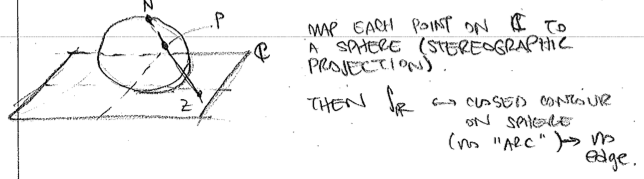
\includegraphics[width=.9\textwidth]{figures/Lec_2017_stereographic.png}
\end{center}
The idea is to place a unit sphere at the origin of $\mathbbm{C}$. The south pole of the sphere is touching $z=0$. Then for any point $z\in\mathbbm{C}$, one can draw a line from $z$ to the north pole of the sphere. There is a single unique point on the sphere that intersects that line. This maps the entire complex plane onto the sphere---except for the north pole of the sphere. We identify the north pole with complex infinity. That's right: all infinities are the same: $\infty$, $i\infty$, $\infty e^{2\pi/3}$, $-\infty$, etc. From this point of view, the real line maps onto the prime meridian of the sphere and there there are no `corners' in the contour. In fact, there's no arc component, either! The integral along the real line is a closed contour with respect to the stereographic projection. Note that the orientation of the contour depends on which hemisphere you are figuratively standing in.

\subsection{The Main Example: follow this carefully}
Let's try another instructive example. Here's an real integral that we would like to solve using contour integral techniques:
\begin{align}
\int dx\, f(x) = \int_{-\infty}^\infty  dx\,
\frac{2\cos x}{x^2+1} \ .
\end{align}
We can analytically continue this into a complex function by simply replacing the real variable with a complex variable, $x\to z$. This complex function $f(z)$ is analytic on the real line. The presence of simple poles at $z=\pm i$ mean that it is meromorphic with respect to the whole complex plane. It is convenient---for reasons that will be clear momentarily---to write the cosine as a sum of exponentials:
\begin{align}
	f(z) 
	= \frac{e^{iz}+e^{-iz}}{(z+i)(z-i)} 
	= \frac{e^{iz}}{(z+i)(z-i)} + \frac{e^{-iz}}{(z+i)(z-i)} 
	\equiv f_+(z) + f_-(z)
	\ .
\end{align}
With some foresight, we have separated $f(z)=f_+(z)+f_-(z)$ into two different functions. 
%
There are now two obvious choices for convenient integration contours that include the real line with the appropriate orientation:
\begin{center}
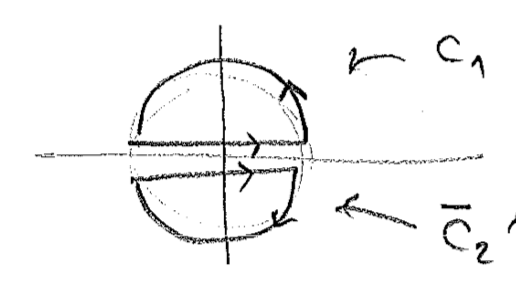
\includegraphics[width=.5\textwidth]{figures/Lec_2017_14_whichcontour.png}
\end{center}
We label the two contours are $C_1$ and $\bar C_2$. The bar over $\bar C_2$ is to remind us of the clockwise orientation; alternatively one could\footnote{This all boils down to notation. You are free to be creative with notation, but the underlying quest is \emph{clarity}. Notation doesn't change the underlying mathematics or physics, but a good notation make your ideas clearer---perhaps even to yourself.} have written $\bar C_2 = -C_2$.  Does it matter which contour we pick?

Our criteria for a convenient contour are that (1) the contour includes the real line with the appropriate orientation and (2) the rest of the contour integrates to zero. That way we can use the residue theorem:
\begin{align}
	\int_C f(z) dz 
	= \int_{-\infty}^\infty dx\, f(x)
	+ \int_{\text{arc}}dz\, f(z) = 
	\int_{-\infty}^\infty dx\, f(x)
	= \sum_{i=\text{poles}}\text{Res}_f(z_i) \ ,
\end{align}
where we recall that $i$ is runs over the poles enclosed by the contour $C$. The condition that the integral over the arc vanishes determines which contour we take. We may conveniently parameterize the arcs as follows:
\begin{align}
	z(\theta) &= R\cos\theta + i R\sin\theta
	\label{eq:z:paramterization:large:arc}
\end{align}
where for $C_1$ the arc is given by $\theta \in [0,\pi]$ while for $\bar C_2$ the arc is $\theta\in[0,-\pi]$. We assume the limit $R\to \infty$. The arc integrals are then:
\begin{align}
	\int_{\text{arc}}
	dz \, 
	%  \left[f_+(z) + f_-(z)\right]
	f_\pm(z)
	=
	\int_\text{arc}
	d\theta \, 
	\frac{e^{\pm iz}}{z^2+1}
	% + 
	% \int_\text{arc}
	% d\theta \, 
	% \frac{e^{iz}}{z^2+1} 
	\ .
\end{align}
When we plug in the parameterization \eqref{eq:z:paramterization:large:arc}, we see that the denominator of $f_\pm$ scales like $R^2$. There's an additional factor of $R$ in the numerator coming from $dz$, and so it may  appear that \emph{either} $C_1$ or $\bar C_2$ could be used. However, recall that $f_{\pm}(z)\sim e^{\pm iz}$ and exponentials beat polynomials. Plugging in $z(\theta)$ into the exponentials gives
\begin{align}
	e^{\pm iz} &= e^{\pm i\left(R\cos\theta + i R\sin\theta\right)} \ ,
\end{align}
where the difference between $C_1$ and $\bar C_2$ is the range (and direction) of $\theta$.
\begin{itemize}
	\item $C_1$ lives in the upper half plane so the imaginary part of $z$ is positive: $R\sin\theta > 0$ \ .
	\item $C_2$ lives in the lower half plane so the imaginary part of $z$ is negative: $R\sin\theta < 0$\ .	
\end{itemize}
This makes it easy to read off the convergence properties of the exponential
\begin{align}
	e^{\pm iz} &= (\text{oscillating})e^{\mp R\sin\theta} \ .
\end{align}
The oscillating part is not relevant: since $|e^{i\varphi}| = 1$ , this factor doesn't actually affect the magnitude of the contribution of the integrand, just the phase. The $\exp(\mp R\sin\theta)$ factor, on the other hand, is everything. 
\begin{itemize}
	\item $e^{- R\sin\theta}$ is exponentially suppressed when $\sin\theta > 0$, this corresponds to the upper half plane and so we use the $C_1$ arc to complete the integration contour of the $f_+(z)\sim \exp(-R\sin\theta)$ integrand.
	\item $e^{+ R\sin\theta}$ is exponentially suppressed when $\sin\theta < 0$, this corresponds to the lower half plane and so we use the $\bar C_2$ arc to complete the integration contour of the $f_-(z)\sim \exp(+R\sin\theta)$ integrand.
\end{itemize}
Because the $e^{-R}$ exponential suppression defeats the polynomial $R^{-1}$ scaling, the vanishing of the integral along the arc is determined only by this exponential factor: $\lim_{R\to\infty}e^{-R}/R\to 0$. We thus have the following approach to the original real integral:
\begin{align}
	\int f(x) &= \int_{-\infty}^\infty  dx\,
\frac{2\cos x}{x^2+1} 
	= 
	\int_{-\infty}^\infty  dx\,
	\frac{e^{+ix}}{x^2+1} 
	+
	\int_{-\infty}^\infty  dx\,
	\frac{e^{-ix}}{x^2+1} 
	\\ 
	&=
	\int_{C_1} dz\, 
	\frac{e^{+iz}}{z^2+1} 
	+
	\int_{\bar C_2} dz\, 
	\frac{e^{-iz}}{z^2+1} 
	\\
	&=
	2\pi i \text{Res}_{f_+}(i)
	-
	2\pi i \text{Res}_{f_-}(-i)
\ .
\end{align}
In the second step we have used the fact that the integral along the real line can be extended by large arcs along $C_1$ or $\bar C_2$ as long as the integral along those arcs vanishes. The residues are straightforward: 
\begin{align}
	\text{Res}_{f_\pm}(\pm i) = \pm \frac{1}{2ie}
\end{align}
so that the final result is
\begin{align}
	\int_{-\infty}^\infty dx\, f(x) &= \frac{2\pi}{e} \ .
\end{align}


 \subsection{A fancy example}

 Here's an example of the residue theorem used to calculate an integral along just the positive real line,
 \begin{align}
 	\int_0^\infty dx\, x^{1/3} F(x) \ .
 \end{align}
 We can trivially analytically continue the integrand by replacing $x\to z$. Let us assume that $F(x)$ is a meromorphic function with poles away from the positive real line. Let us further assume further that $F(z)$ is exponentially suppressed for $|z| = R \gg 1$, say $F(z)\sim e^{-R}$. Note that the $x^{1/3} \to z^{1/3}$ factor is problematic. It tells us that there's an \emph{branch cut} in our integrand: if we start at some point and went a full circle around the origin, say $z(\theta) = e^{i\theta}$ for $\theta\in[0,2\pi]$, then $z^{1/3}$ doesn't return to the origin. This means you probably need to extend the complex plane into Riemann sheets. Practically what this means is that we have to pick a branch cut that prevents us from taking contours that are `full circles' around the origin. We have the freedom to pick the orientation of this branch cut, but in this case it is convenient to pick it along the positive real line\footnote{If you want to be careful to make sure that you're not interfering with the original integral, you can put the branch cut just below the real line by some vanishingly small amount and take that amount to zero at the end of the calculation.}. Let's take a peculiar contour that includes the integration region we want, $x\in [0,\infty)$, then circles the entire complex plane, and returns back to zero along $x\in (\infty, 0]$. 
 \begin{center}
 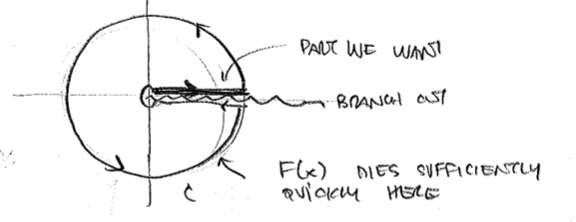
\includegraphics[width=.8\textwidth]{figures/Lec_2017_14_branch.png}
 \end{center}
 In the past, we'd have said that the integral along $x\in [0, \infty)$ should cancel that from $x\in (\infty, 0]$. However, we now notice that there's a branch cut separating those two regions. Indeed, you may already see that the \emph{integrand} is not identical along those two lines. 

Construct the following contour integral:
 \begin{align}
 	\oint_C  dz\, z^{1/3} F(z) &= 
 	\int_0^\infty dx x^{1/3}F(x)
 	+ \int_{\text{arc}} dz \, z^1/3 F(z)
 	+ \int_\infty^0 dx \left(x e^{2\pi i}\right)^{1/3} F\left(e^{2\pi i}\right) \ .
 \end{align}
 The left-hand side is simple to evaluate with the residue theorem and will depend on the poles of the unspecified function $F(z)$. On the right-hand side, the integral along the arc vanishes by the assumptions we've made about $F(z)$ becoming exponentially small for large arguments, $|z|=R\gg 1$.  Finally, we notice that the third term on the right-hand side we've written $z=xe^{2\pi i}$; this is critical since it includes the phase that $z$ picks up when traversing the large circular path. Since $F(z)$ is meromorphic, we may simply replace $F(x\exp(2\pi i)) \to F(x)$. However, the $z^{1/3}$ needs some care. We find:
 \begin{align}
 	2\pi i \sum_{j=\text{poles}} z_j^{1/3} \text{Res}_F (z_j)
 	=
 	\left(1-e^{2\pi i/3}\right) \int_0^\infty dx\,  x^{1/3} F(x) \ .
 \end{align}
The $-e^{2\pi i/3}$ came from the $1/3$-power of the phase. The minus sign comes from $\int_{\infty}^0 dx = -\int_0^\infty dx$. Converting the difference of exponentials into a sine gives
\begin{align}
	\left(1-e^{2\pi i/3}\right) 
	= 2e^{i\pi/3} \cdot \frac{1}{2}\left(e^{-i\pi/3}-e^{i\pi/3}\right)
	= -2 e^{i\pi/3} \sin(\pi/3) \ .
\end{align}
We thus find an expression for the original integral:
\begin{align}
	\int_0^\infty dx\, x^{1/3}F(x) &=
	\sum_{j=\text{poles}}
	\frac{\pi i e^{i\pi/3} z_j^{1/3}\text{Res}_F(z_j)}{\sin(\pi/3)}
	\ .
\end{align}
We won't worry too much about branch cuts in this course. However, they do occasionally show up in physical manifestations, such as in dispersion relations\footnote{See, e.g., \url{https://arxiv.org/abs/1610.06090} for a peek at how it can show up in quantum field theory.}.




